\documentclass{article}

\usepackage{etoolbox}
\newtoggle{arxiv}
\toggletrue{arxiv}




\iftoggle{arxiv}{}{
\PassOptionsToPackage{numbers,sort,compress}{natbib}
\usepackage{neurips_2024}
}







\usepackage[utf8]{inputenc} %
\usepackage[T1]{fontenc}    %
\usepackage{hyperref}       %
\usepackage{url}            %
\usepackage{booktabs}       %
\usepackage{amsfonts}       %
\usepackage{nicefrac}       %
\usepackage{microtype}      %
\usepackage{xcolor}         %
\usepackage{amsmath,amsthm,amssymb}

\usepackage{algorithm}
\usepackage{algorithmic}

\usepackage{caption}
\captionsetup[figure]{font=small}
\usepackage{subcaption}
\usepackage{multirow}

\usepackage{xspace}
\usepackage{wrapfig}

\usepackage{pifont}
\newcommand{\xmark}{\ding{55}}

\usepackage[capitalise]{cleveref}  %

\crefname{section}{\S\hspace{-0.2em}}{\S\S\hspace{-0.2em}}
\crefname{subsection}{\S\hspace{-0.2em}}{\S\S\hspace{-0.2em}}
\crefname{subsubsection}{\S\hspace{-0.2em}}{\S\S\hspace{-0.2em}}

\usepackage{comment}
\usepackage[inline]{enumitem}

\usepackage{graphicx}
\usepackage{grffile}
\usepackage{color}

\usepackage{newtxmath}

\iftoggle{arxiv}{
\usepackage[numbers,sort]{natbib}
}{}

\usepackage{import}

\usepackage{tikz-cd}
\usepackage{tikz}

\providecommand{\main}{.}

\newtoggle{todo}
\toggletrue{todo}
\newcommand{\todo}[1]{\iftoggle{todo}{\textcolor{cyan}{[TODO: #1]}}{}}

\newtoggle{comment}
\togglefalse{comment} %
\newcommand{\TD}[1]{\iftoggle{comment}{\textcolor{magenta}{[TD: #1]}}{}}


\renewcommand{\max}{\mathrm{max}}
\renewcommand{\exp}{\mathrm{exp}}
\newcommand{\abs}[1]{\left\lvert#1\right\rvert}
\newcommand{\norm}[1]{\left\|{#1}\right\|} %
\newcommand{\diag}{\mathrm{diag}}
\newcommand{\softmax}{\mathrm{softmax}}
\newcommand{\rowmax}{\mathrm{rowmax}}
\newcommand{\rowsum}{\mathrm{rowsum}}
\newcommand{\dsoftmax}{\mathrm{dsoftmax}}
\providecommand{\tr}{\mathop{\rm tr}}

\newcommand{\defeq}{:=}

\newcommand{\RR}{\mathbb{R}}

\newcommand{\vQ}{\mathbf{Q}}
\newcommand{\vK}{\mathbf{K}}
\newcommand{\vV}{\mathbf{V}}
\newcommand{\vdQ}{\mathbf{dQ}}
\newcommand{\vdK}{\mathbf{dK}}
\newcommand{\vdV}{\mathbf{dV}}
\newcommand{\vS}{\mathbf{S}}
\newcommand{\vdS}{\mathbf{dS}}
\newcommand{\vP}{\mathbf{P}}
\newcommand{\vdP}{\mathbf{dP}}
\newcommand{\vU}{\mathbf{U}}
\newcommand{\vW}{\mathbf{W}}
\newcommand{\vT}{\mathbf{T}}
\newcommand{\vX}{\mathbf{X}}
\newcommand{\vO}{\mathbf{O}}
\newcommand{\vdO}{\mathbf{dO}}
\newcommand{\vM}{\mathbf{M}}
\newcommand{\vZ}{\mathbf{Z}}

\newcommand{\fa}{\textsc{FlashAttention}\xspace}
\newcommand{\sysnameone}{\textsc{FlashAttention}\xspace}
\newcommand{\faa}{\textsc{FlashAttention-2}\xspace}
\newcommand{\fat}{\textsc{FlashAttention-3}\xspace}  %

\newtheorem{theorem}{Theorem}
\newtheorem*{theorem*}{Theorem}
\newtheorem{corollary}[theorem]{Corollary}
\newtheorem{definition}{Definition}
\newtheorem{lemma}[theorem]{Lemma}
\newtheorem{claim}[theorem]{claim}
\newtheorem{example}{Example}
\newtheorem{proposition}[theorem]{Proposition}


\newcommand*\samethanks[1][\value{footnote}]{\footnotemark[#1]}
\usepackage{authblk}
\makeatletter
\renewcommand\AB@affilsepx{ \protect\Affilfont}
\makeatother

\iftoggle{arxiv}{
  \setlength{\textwidth}{6.9in}
  \setlength{\textheight}{9in}
  \setlength{\oddsidemargin}{0in}
  \setlength{\evensidemargin}{0in}
  \setlength{\topmargin}{-0.5in}
  \newlength{\defbaselineskip}
  \setlength{\defbaselineskip}{\baselineskip}
  \setlength{\marginparwidth}{0.8in}
}{
\usepackage[compact]{titlesec}
\titlespacing{\section}{0pt}{*1}{*0}
\titlespacing{\subsection}{0pt}{*1.5}{*0}

\usepackage[subtle, mathdisplays=normal, charwidths=normal, leading=normal]{savetrees}

\addtolength\textfloatsep{-0.5em}
\addtolength\intextsep{-0.2em}


\def\setstretch#1{\renewcommand{\baselinestretch}{#1}}
\setstretch{0.985}
\addtolength{\parskip}{-1pt}

}

\title{FlashAttention-3:\\ Fast and Accurate Attention with Asynchrony and Low-precision}

\iftoggle{arxiv}{
  \author[$^1$]{Jay Shah\thanks{Equal contribution}}
  \author[$^1$]{Ganesh Bikshandi\samethanks}
  \author[$^2$]{Ying Zhang}
  \author[$^{3,4}$]{Vijay Thakkar}
  \author[$^3$]{Pradeep Ramani}
  \author[$^{5,6}$]{Tri Dao}
  \affil[$^1$]{Colfax Research}
  \affil[$^2$]{Meta}
  \affil[$^3$]{NVIDIA}
  \affil[$^4$]{Georgia Tech}
  \affil[$^5$]{Princeton University}
  \affil[$^6$]{Together AI\newline}
  \affil[ ]{\hspace{-2em}{\small\texttt{\{jayhshah,ganesh\}@colfax-intl.com},
      \texttt{yingz@meta.com}, \texttt{\{vithakkar,prraman\}@nvidia.com}, \texttt{tri@tridao.me}}}
}{



\author{%
  Jay Shah\thanks{Equal contribution}\: $^{1}$,
  Ganesh Bikshandi\samethanks\: $^{1}$, Ying Zhang $^{2}$, Vijay Thakkar $^{3,4}$,
  Pradeep Ramani $^{3}$, Tri Dao$^{8,9}$\\
  $^1$ Colfax Research\\
  $^2$ Meta\\
  $^3$ NVIDIA \\
  $^4$ Georgia Institute of Technology\\
  $^8$ Princeton University\\
  $^9$ Together AI\\
  {\small\texttt{\{tri\}@tridao.me}}
}
}

\begin{document}


\maketitle


\begin{abstract}
Scaling Transformers to longer sequence lengths has been a major problem in the
last several years, promising to improve performance in language modeling and
high-resolution image understanding, as well as to unlock new applications in
code, audio, and video generation.
The attention layer is the main bottleneck in scaling to longer sequences, as
its runtime and memory increase quadratically in the sequence length.
\sysnameone~\citep{dao2022flashattention} exploits the asymmetric GPU memory
hierarchy to bring significant memory saving (linear instead of quadratic) and
runtime speedup (2-4$\times$ compared to optimized baselines), with no approximation.
However, \sysnameone is still not nearly as fast as optimized matrix-multiply
(GEMM) operations, reaching only 25-40\% of the theoretical maximum FLOPs/s.
We observe that the inefficiency is due to suboptimal work partitioning between
different thread blocks and warps on the GPU, causing either low-occupancy or
unnecessary shared memory reads/writes.
We propose \sysname, with better work partitioning to address these issues.
In particular, we (1) tweak the algorithm to reduce the number of non-matmul
FLOPs (2) parallelize the attention computation, even for a single head, across
different thread blocks to increase occupancy, and (3) within each thread block,
distribute the work between warps to reduce communication through shared memory.
These yield around 2$\times$ speedup compared to \sysnameone, reaching 50-73\% of the
theoretical maximum FLOPs/s on A100 and getting close to the efficiency of GEMM
operations.
We empirically validate that when used end-to-end to train GPT-style models,
\sysname reaches training speed of up to 225 TFLOPs/s per A100 GPU (72\% model
FLOPs utilization).\footnote{\sysname
  is available at \url{https://github.com/Dao-AILab/flash-attention}}

% models with up to 2$\times$ longer sequence length compared to \sysnameone, in the
% same amount of time, leading to better downstream performance.\footnote{\sysname
%   is available at \url{https://github.com/Dao-AILab/flash-attention}}

\end{abstract}


\documentclass[11pt]{report}
\usepackage[margin=2cm]{geometry}
\usepackage{graphicx}
\usepackage{float}
\usepackage{times}
\usepackage{url}
\usepackage[dvipsnames]{xcolor}
\usepackage{hyperref}

\newcommand{\specialcell}[2][c]{\begin{tabular}[#1]{@{}c@{}}#2\end{tabular}}

\newcommand{\Gap}{\texorpdfstring{\hfill}{}}
\newcommand{\Rec}{\texorpdfstring{{\small\emph{\color{ccai-blue}{\fbox{High Leverage}}}}}{}}
\newcommand{\HighRisk}{\texorpdfstring{{\small\emph{\color{ccai-yellow-darker}{\fbox{Uncertain Impact}}}}}{}}
\newcommand{\Longterm}{\texorpdfstring{{\small\emph{\color{ccai-green}{\fbox{Long-term}}}}}{}}

\begin{document}

\begin{abstract}
Climate change is one of the greatest challenges facing humanity, and we, as machine learning experts, may wonder how we can help. Here we describe how machine learning can be a powerful tool in reducing greenhouse gas emissions and helping society adapt to a changing climate. From smart grids to disaster management, we identify high impact problems where existing gaps can be filled by machine learning, in collaboration with other fields. Our recommendations encompass exciting research questions as well as promising business opportunities. We call on the machine learning community to join the global effort against climate change.
\vskip .5in
\end{abstract}

\part*{Introduction}
The effects of climate change are increasingly visible.\footnote{For a layman's introduction to the topic of climate change, see \cite{romm2018climate, archer2010climate}.} Storms, droughts, fires, and flooding have become stronger and more frequent \cite{field2012managing}. Global ecosystems are changing, including the natural resources and agriculture on which humanity depends. The 2018 intergovernmental report on climate change estimated that the world will face catastrophic consequences unless global greenhouse gas emissions are eliminated within thirty years \cite{ipcc_global_2018}. Yet year after year, these emissions rise.

Addressing climate change involves mitigation (reducing emissions) and adaptation (preparing for unavoidable consequences). Both are multifaceted issues. Mitigation of greenhouse gas (GHG) emissions requires changes to electricity systems, transportation, buildings, industry, and land use. Adaptation requires planning for resilience and disaster management, given an understanding of climate and extreme events. Such a diversity of problems can be seen as an opportunity: there are many ways to have an impact.

In recent years, machine learning (ML) has been recognized as a broadly powerful tool for technological progress. Despite the growth of movements applying ML and AI to problems of societal and global good,\footnote{See the AI for social good movement (e.g.~\cite{hager2019artificial, berendt2019ai}), ML for the developing world~\cite{de2018machine}, the computational sustainability movement (e.g.~\cite{kelling2018computational, joppa2017case, lassig2016computational, gomes2009computational, dietterich2009machine}, the American Meteorological Society's Committee on AI Applications to Environmental Science, and the field of Climate Informatics (\url{www.climateinformatics.org}) \cite{Monteleoni2013chapter}, as well as the relevant survey papers \cite{faghmous2014big, kaack2019challenges, ford2016opinion}.} there remains the need for a concerted effort to identify how these tools may best be applied to tackle climate change. Many ML practitioners wish to act, but are uncertain how. On the other side, many fields have begun actively seeking input from the ML community.

This paper aims to provide an overview of where machine learning can be applied with high impact in the fight against climate change, through either effective engineering or innovative research. The strategies we highlight include climate mitigation and adaptation, as well as meta-level tools that enable other strategies. In order to maximize the relevance of our recommendations, we have consulted experts across many fields (see \hyperref[sec:acknowledgments]{{\small{Acknowledgments}}}) in the preparation of this paper.


\begin{table}
\begin{small}
\begin{center}
\begin{tabular}{l l l l l l l l l l l l}  \toprule
     \multicolumn{2}{l}{ }
         & \small{\rotatebox{90}{\parbox{2.2cm}{Causal\\inference}}}
         & \small{\rotatebox{90}{\parbox{2.2cm}{Computer\\vision}}}
         & \small{\rotatebox{90}{\parbox{2.2cm}{Interpretable\\models}}}
         & \small{\rotatebox{90}{NLP}}
         & \small{\rotatebox{90}{\parbox{2.2cm}{RL \& Control}}}
        %  & \small{\rotatebox{90}{Robotics}}
         & \small{\rotatebox{90}{\parbox{2.2cm}{Time-series analysis}}}
         & \small{\rotatebox{90}{\parbox{2.2cm}{Transfer\\learning}}}
         & \small{\rotatebox{90}{\parbox{2.2cm}{Uncertainty\\quantification}}}
         & \small{\rotatebox{90}{\parbox{2.2cm}{Unsupervised\\learning}}}
    \\ \midrule
    \rowcolor{ccai-blue-lightest}
    \multicolumn{2}{l}{1 \hyperref[sec:electricity-systems]{Electricity systems}} 
        & % Causal inf
        &  % Comp vision
        & % Interpretable ml
        & % nlp
        & % rl + control
        & % time series
        & % transfer
        & % UQ
        & \\% unsupervised \ref{sub
    & \hyperref[sec:electricity-lowCarbon]{Enabling low-carbon electricity}
        & % Causal inf
        & $\bullet$% Comp vision
        & $\bullet$% % Interpretable ml
        & % % nlp
        & $\bullet$%% rl + control
        & $\bullet$% % time series
        & % transfer
        & $\bullet$% % UQ
        & $\bullet$\\% unsupervised 
    & \hyperref[sec:electricity-currentSystemImpact]{Reducing current-system impacts}
        & % Causal inf
        & $\bullet$% Comp vision
        & % Interpretable ml
        & % nlp
        & % rl + control
        & $\bullet$% % time series
        & % transfer
        & $\bullet$% % UQ
        & $\bullet$\\% unsupervised 
    & \hyperref[sec:electricity-developing]{Ensuring global impact}
        & % Causal inf
        & $\bullet$% Comp vision
        & % Interpretable ml
        & % nlp
        & % rl + control
        & % time series
        & $\bullet$ % transfer
        & % UQ
        & $\bullet$\\% unsupervised 
    \rowcolor{ccai-blue-lightest}
    \multicolumn{2}{l}{2 \hyperref[sec:transportation]{Transportation}} 
        & % Causal inf
        & % Comp vision
        &% Interpretable ml
        & % nlp
        & % rl + control
        & % time series
        & % transfer
        & % UQ
        & \\% unsupervised 
    & \hyperref[sec:TReducing]{Reducing transport activity}
        & % Causal inf
        & $\bullet$% Comp vision
        & % Interpretable ml
        & % nlp
        & % rl + control
        & $\bullet$% time series
        & % transfer
        & $\bullet$% UQ
        & $\bullet$\\% unsupervised     
   & \hyperref[sec:TEfficient]{Improving vehicle efficiency}
        & % Causal inf
        & $\bullet$% Comp vision
        & % Interpretable ml
        & % nlp
        & $\bullet$% rl + control
        & % time series
        & % transfer
        & % UQ
        & \\% unsupervised    
   & \hyperref[sec:TFuels]{Alternative fuels \& electrification}
        & % Causal inf
        & % Comp vision
        & % Interpretable ml
        & % nlp
        & $\bullet$% rl + control
        & % time series
        & % transfer
        & % UQ
        & $\bullet$ \\% unsupervised    
   & \hyperref[sec:modalshift]{Modal shift}
        & $\bullet$% Causal inf
        & $\bullet$% Comp vision
        & % Interpretable ml
        & % nlp
        & % rl + control
        & $\bullet$% time series
        & % transfer
        & $\bullet$% UQ
        & \\% unsupervised    
    \rowcolor{ccai-blue-lightest}
    \multicolumn{2}{l}{3 \hyperref[sec:buildings-cities]{Buildings and cities}} 
        & % Causal inf
        & % Comp vision
        & % Interpretable ml
        & % nlp
        & % rl + control
        & % time series
        & % transfer
        & % UQ
        & \\% unsupervised 
    & \hyperref[sec:indv]{Optimizing buildings}
        & $\bullet$% Causal inf
        & % Comp vision
        & % Interpretable ml
        & % nlp
        & $\bullet$% rl + control
        & $\bullet$% time series
        & $\bullet$% transfer
        & % UQ
        & \\% unsupervised 
    & \hyperref[sec:distr]{Urban planning}
        & % Causal inf
        & $\bullet$% Comp vision
        & % Interpretable ml
        & % nlp
        & % rl + control
        & $\bullet$% time series
        & $\bullet$% transfer
        & % UQ
        & $\bullet$\\% unsupervised 
    & \hyperref[sec:cities]{The future of cities}
        & % Causal inf
        & % Comp vision
        & % Interpretable ml
        & $\bullet$%% nlp
        & % rl + control
        & %% time series
        & $\bullet$%% transfer
        & $\bullet$% UQ
        & $\bullet$\\% unsupervised 
    \rowcolor{ccai-blue-lightest}
    \multicolumn{2}{l}{4 \hyperref[sec:industry]{Industry}} 
        & % Causal inf
        & % Comp vision
        & % Interpretable ml
        & % nlp
        & % rl + control
        & % time series
        & % transfer
        & % UQ
        & \\% unsupervised 
    & \hyperref[sec:supplychains]{Optimizing supply chains}
        & % Causal inf
        & $\bullet$ %% Comp vision
        & % Interpretable ml
        & % nlp
        & $\bullet$ % rl + control
        & $\bullet$ % time series
        & % transfer
        & % UQ
        & \\% unsupervised 
    & \hyperref[sec:materialsandconstruction]{Improving materials}
        & %% Causal inf
        & % Comp vision
        & % Interpretable ml
        & % nlp
        & % rl + control
        & % time series
        & %% transfer
        & % UQ
        & $\bullet$ \\% unsupervised 
    & \hyperref[sec:demandresponse]{Production \& energy}
        & %% Causal inf
        & $\bullet$%% Comp vision
        & $\bullet$ %% Interpretable ml
        & % nlp
        & $\bullet$% rl + control
        & %% time series
        & %% transfer
        & % UQ
        & \\% unsupervised 
    \rowcolor{ccai-blue-lightest}
    \multicolumn{2}{l}{5 \hyperref[sec:afolu]{Farms \& forests}} 
        & % Causal inf
        & % Comp vision
        & % Interpretable ml
        & % nlp
        & % rl + control
        & % time series
        & % transfer
        & % UQ
        & \\% unsupervised 
    & \hyperref[sec:emissions-detection]{Remote sensing of emissions}
        & % Causal inf
        & $\bullet$% Comp vision
        & % Interpretable ml
        & % nlp
        & % rl + control
        & % time series
        & % transfer
        & % UQ
        & \\% unsupervised 
    & \hyperref[sec:agriculture]{Precision agriculture}
        & % Causal inf
        & $\bullet$% Comp vision
        & % Interpretable ml
        & % nlp
        & $\bullet$% rl + control
        & $\bullet$% time series
        & % transfer
        & % UQ
        & \\% unsupervised 
    & \hyperref[sec:peatlands]{Monitoring peatlands}
        & % Causal inf
        & $\bullet$% Comp vision
        & % Interpretable ml
        & % nlp
        & % rl + control
        & % time series
        & % transfer
        & % UQ
        & \\% unsupervised 
    & \hyperref[sec:forests]{Managing forests}
        & % Causal inf
        & $\bullet$% Comp vision
        & % Interpretable ml
        & % nlp
        & $\bullet$ % rl + control
        & $\bullet$ % time series
        & % transfer
        & % UQ
        & \\% unsupervised 
    \rowcolor{ccai-blue-lightest}
    \multicolumn{2}{l}{6 \hyperref[sec:ccs]{Carbon dioxide removal}}
        & % Causal inf
        & % Comp vision
        & % Interpretable ml
        & % nlp
        & % rl + control
        & % time series
        & % transfer
        & % UQ
        & \\
    & \hyperref[sec:ccs]{Direct air capture}
        & % Causal inf
        & % Comp vision
        & % Interpretable ml
        & % nlp
        & % rl + control
        & % time series
        & % transfer
        & % UQ
        & $\bullet$\\% unsupervised 
    & \hyperref[subsubsec: sequestrativervin]{Sequestering~\cd}
        & % Causal inf
        & $\bullet$% Comp vision
        & % Interpretable ml
        & % nlp
        & % rl + control
        & % time series
        & % transfer
        & $\bullet$% UQ
        & $\bullet$\\% unsupervised 
    \rowcolor{ccai-blue-lightest}
    \multicolumn{2}{l}{7 \hyperref[sec: climate prediction]{Climate prediction}} 
        & % Causal inf
        & % Comp vision
        & % Interpretable ml
        & % nlp
        & % rl + control
        & % time series
        & % transfer
        & % UQ
        & \\% unsupervised 
    & \hyperref[sec:climate-models-params]{Uniting data, ML \& climate science}
        & % Causal inf
        & $\bullet$% Comp vision
        & $\bullet$% Interpretable ml
        & % nlp
        & % rl + control
        & $\bullet$% time series
        & % transfer
        & $\bullet$% UQ
        & \\% unsupervised 
    & \hyperref[sec:models-extreme-events]{Forecasting extreme events}
        & % Causal inf
        & $\bullet$% Comp vision
        & $\bullet$% Interpretable ml
        & % nlp
        & % rl + control
        & $\bullet$% time series
        & % transfer
        & $\bullet$% UQ
        & \\% unsupervised 
    \rowcolor{ccai-blue-lightest}
    \multicolumn{2}{l}{8 \hyperref[sec:societal-impacts]{Societal impacts}} 
        & % Causal inf
        & % Comp vision
        & % Interpretable ml
        & % nlp
        & % rl + control
        & % time series
        & % transfer
        & % UQ
        & \\% unsupervised 
    & \hyperref[subsub:ecology]{Ecology}
        & % Causal inf
        & $\bullet$% Comp vision
        & % Interpretable ml
        & % nlp
        & % rl + control
        & % time series
        & $\bullet$% transfer
        & % UQ
        & \\% unsupervised 
    & \hyperref[subsub:infrastructure]{Infrastructure}
        & % Causal inf
        & % Comp vision
        & % Interpretable ml
        & % nlp
        & $\bullet$% rl + control
        & $\bullet$% time series
        & % transfer
        & $\bullet$% UQ
        & \\% unsupervised 
    & \hyperref[subsub:social_systems]{Social systems}
        & % Causal inf
        & $\bullet$% Comp vision
        & % Interpretable ml
        & % nlp
        & % rl + control
        & $\bullet$% time series
        & % transfer
        & % UQ
        & $\bullet$\\% unsupervised 
    & \hyperref[subsub:crisis]{Crisis}
        & % Causal inf
        & $\bullet$% Comp vision
        & % Interpretable ml
        & $\bullet$% nlp
        & % rl + control
        & % time series
        & % transfer
        & % UQ
        & \\% unsupervised 
    \rowcolor{ccai-blue-lightest}
    \multicolumn{2}{l}{9 \hyperref[sec:geoengineering]{Solar geoengineering}} 
        & % Causal inf
        & % Comp vision
        & % Interpretable ml
        & % nlp
        & % rl + control
        & % time series
        & % transfer
        & % UQ
        & \\% unsupervised 
    & \hyperref[subsub:better-aerosols]{Understanding \& improving aerosols}
        & % Causal inf
        & % Comp vision
        & % Interpretable ml
        & % nlp
        & % rl + control
        & $\bullet$% time series
        & % transfer
        & $\bullet$% UQ
        & \\% unsupervised 
    & \hyperref[subsub:planetary-control]{Engineering a planetary control system}
        & % Causal inf
        & % Comp vision
        & % Interpretable ml
        & % nlp
        & $\bullet$% rl + control
        & % time series
        & % transfer
        & $\bullet$% UQ
        & \\% unsupervised 
    & \hyperref[subsub:impact-models]{Modeling impacts}
        & % Causal inf
        & % Comp vision
        & % Interpretable ml
        & % nlp
        & % rl + control
        & $\bullet$% time series
        & % transfer
        & $\bullet$% UQ
        & \\% unsupervised 
    \rowcolor{ccai-blue-lightest}
    \multicolumn{2}{l}{10 \hyperref[sec:tools-individuals]{Individual action}} 
        & % Causal inf
        & % Comp vision
        & % Interpretable ml
        & % nlp
        & % rl + control
        & % time series
        & % transfer
        & % UQ
        & \\% unsupervised 
    & \hyperref[sec:personal_carbon_footprint]{Understanding personal footprint}
        & $\bullet$% Causal inf
        & % Comp vision
        & % Interpretable ml
        & $\bullet$% nlp
        & $\bullet$% rl + control
        & $\bullet$% time series
        & % transfer
        & % UQ
        & \\% unsupervised 
    & \hyperref[sec:behavior_change]{Facilitating behavior change}
        & % Causal inf
        & % Comp vision
        & % Interpretable ml
        & $\bullet$% nlp
        & % rl + control
        & % time series
        & % transfer
        & % UQ
        & $\bullet$\\% unsupervised 
    \rowcolor{ccai-blue-lightest}
    \multicolumn{2}{l}{11 \hyperref[sec:toolsforsociety]{Collective decisions}} 
        & % Causal inf
        & % Comp vision
        & % Interpretable ml
        & % nlp
        & % rl + control
        & % time series
        & % transfer
        & % UQ
        &  \\% unsupervised 
    & \hyperref[sec:coordination]{Modeling social interactions}
        & % Causal inf
        & % Comp vision
        & $\bullet$ % Interpretable ml
        & % nlp
        & $\bullet$ % rl + control
        & % time series
        & % transfer
        & % UQ
        & \\% unsupervised 
    & \hyperref[sec:decisionmaking]{Informing policy}
        & $\bullet$ % Causal inf
        & $\bullet$ % Comp vision
        & % Interpretable ml
        & $\bullet$% nlp
        & % rl + control
        & % time series
        & % transfer
        & $\bullet$% UQ
        & $\bullet$\\% unsupervised 
    & \hyperref[subsec:markets]{Designing markets}
        & % Causal inf
        & % Comp vision
        & % Interpretable ml
        & % nlp
        & $\bullet$% rl + control
        & $\bullet$% time series
        & % transfer
        & % UQ
        & $\bullet$\\% unsupervised 
    \rowcolor{ccai-blue-lightest}
    \multicolumn{2}{l}{12 \hyperref[sec:education]{Education}} 
        & % Causal inf
        & % Comp vision
        & % Interpretable ml
        & $\bullet$% nlp
        & $\bullet$% rl + control
        & % time series
        & % transfer
        & % UQ
        & \\% unsupervised 
    \rowcolor{ccai-blue-lightest}
    \multicolumn{2}{l}{13 \hyperref[sec:finance]{Finance}} 
        & % Causal inf
        & % Comp vision
        & % Interpretable ml
        & $\bullet$% nlp
        & % rl + control
        & $\bullet$% time series
        & % transfer
        & $\bullet$% UQ
        & \\% unsupervised 
    \bottomrule
\end{tabular}
\caption{Climate change solution domains, corresponding to sections of this paper, matched with selected areas of ML that are relevant to each. }
\label{tab:summary}
\end{center}
\end{small}
\end{table}


\subsection*{Who is this paper written for?}

We believe that our recommendations will prove valuable to several different audiences (detailed below). In our writing, we have assumed some familiarity with basic terminology in machine learning, but do not assume any prior familiarity with application domains (such as agriculture or electric grids).\\

\textbf{Researchers and engineers:}
We identify many problems that require conceptual innovation and can advance the field of ML, as well as being highly impactful. For example, we highlight how climate models afford an exciting domain for interpretable ML (see \S\ref{sec: climate prediction}).
We encourage researchers and engineers across fields to use their expertise in solving urgent problems relevant to society.\\

\textbf{Entrepreneurs and investors:} We identify many problems where existing ML techniques could have a major impact without further research, and where the missing piece is deployment. We realize that some of the recommendations we offer here will make valuable startups and nonprofits. For example, we highlight techniques for providing fine-grained solar forecasts for power companies (see \S\ref{sec:electricity-lowCarbon}), tools for helping reduce personal energy consumption (see \S\ref{sec:behavior_change}), and predictions for the financial impacts of climate change (see \S\ref{sec:finance}). We encourage entrepreneurs and investors to fill what is currently a wide-open space.\\

\textbf{Corporate leaders:} We identify problems where ML can lead to massive efficiency gains if adopted at scale by corporate players. For example, we highlight means of optimizing supply chains to reduce waste (see \S\ref{sec:supplychains}) and software/hardware tools for precision agriculture (see \S\ref{sec:agriculture}). We encourage corporate leaders to take advantage of opportunities offered by ML to benefit both the world and the bottom line.\\

\textbf{Local and national governments:} We identify problems where ML can improve public services, help gather data for decision-making, and guide plans for future development. For example, we highlight intelligent transportation systems (see \S\ref{sec:modalshift}), techniques for automatically assessing the energy consumption of buildings in cities (see \S\ref{sec:indv}),
and tools for improving disaster management (see \S\ref{subsub:crisis}). We encourage governments to consult ML experts while planning infrastructure and development, as this can lead to better, more cost-effective outcomes. We further encourage public entities to release data that may be relevant to climate change mitigation and adaptation goals.\\

\subsection*{How to read this paper} \label{sub:howtoread}
The paper is broken into sections according to application domain (see Table \ref{tab:summary}). To help the reader, we have also included the following flags at the level of individual strategies.
\begin{itemize}
\item \textbf{\Rec} $\,$ denotes bottlenecks that domain experts have identified in climate change mitigation or adaptation and that we believe to be particularly well-suited to tools from ML. These areas may be especially fruitful for ML practitioners wishing to have an outsized impact, though applications not marked with this flag are also valuable and should be pursued.
\item \textbf{\Longterm} $\,$ denotes applications that will have their primary impact after 2040. While extremely important, these may in some cases be less pressing than those which can help act on climate change in the near term.
\item \textbf{\HighRisk} $\,$ denotes applications where the impact on GHG emissions is uncertain (for example, the \emph{Jevons paradox} may apply\footnote{The Jevons paradox in economics refers to a situation where increased efficiency nonetheless results in higher overall demand. For example, autonomous vehicles could cause people to drive far more, so that overall GHG emissions could increase even if each ride is more efficient. In such cases, it becomes especially important to make use of specific policies, such as carbon pricing, to direct new technologies and the ML behind them. See also the literature on rebound effects and induced demand.}) or where there is  potential for undesirable side effects (\emph{negative externalities}).
\end{itemize}

These flags should not be taken as definitive; they represent our understanding of more rigorous analyses within the domains we consider, combined with our subjective evaluation of the potential role of ML in these various applications.

Despite the length of the paper, we cannot cover everything. There will certainly be many applications that we have not considered, or that we have erroneously dismissed. We look forward to seeing where future work leads.

\subsection*{A call for collaboration}

All of the problems we highlight in this paper require collaboration across fields. As the language used to refer to problems often varies between disciplines, we have provided keywords and background reading within each section of the paper. Finding collaborators and relevant data can sometimes be difficult; for additional resources, please visit the website that accompanies this paper: \url{https://www.climatechange.ai/}.

Collaboration makes it easier to develop effective strategies. Working with domain experts reduces the chance of using powerful tools when simple tools will do the job, of working on a problem that isn't actually relevant to practitioners, of overly simplifying a complex issue,
or of failing to anticipate risks.

Collaboration can also help ensure that new work reaches the audience that will use it. To be impactful, ML code should be accessible and published using a language and a platform that are already popular with the intended users. For maximal impact, new code can be integrated into an existing, widely used tool.

We emphasize that machine learning is not a silver bullet. The applications we highlight are impactful, but no one solution will ``fix'' climate change. There are also many areas of action where ML is inapplicable, and we omit these entirely. Furthermore, technology alone is not enough -- technologies that would address climate change have been available for years, but have largely not been adopted at scale by society. While we hope that ML will be useful in reducing the costs associated with climate action, humanity also must decide to act.

\end{document}


\subsection{Data Augmentation in NLP}
The problem of domain adaptation and OOD robustness is well established in NLP \citep{blitzer-etal-2007-biographies,daume-iii-2007-frustratingly,hendrycks2020pretrained}.
Existing work on improving generalization has focused on data augmentation, where synthetically generated training examples are used to augment an existing dataset.
It is hypothesized that these examples induce robustness to local perturbations, which has been shown to be effective in semi-supervised and self-supervised settings \citep{bachman2014learning,szegedy2014intriguing, sajjadi2016regularization}.

Existing task-specific methods \citep{kafle-etal-2017-data} and word-level methods \citep{zhang2015character, xie2017data, wei-zou-2019-eda} are based on human-designed heuristics.
Back-translation from or through another language has been applied in the context of machine translation \citep{sennrich2016improving}, question answering \citep{wei2018fast}, and consistency training \citep{xie2019unsupervised}.
More recent work has used word embeddings \citep{wangyang2015thats} and LSTM language models \citep{fadaee2017data} to perform word replacement.
Other methods focus on fine-tuning contextual language models \citep{kobayashi-2018-contextual,wu2019conditional,kumar20202data} or large generative models \citep{lambada,yang2020g-daug,kumar20202data} to generate synthetic examples.

\subsection{VRM and the Manifold Assumption}
Vicinal Risk Minimization (VRM) \citep{vicinal200olivier} formalizes data augmentation as enlarging the training set support by drawing samples from a \textit{vicinity} of existing training examples.
Typically the vicinity of a training example is defined using dataset-dependent heuristics.
For example, in computer vision, examples are generated using scale augmentation \citep{simonyan2014very}, color augmentation \citep{krizhevsky2012imagenet}, and translation and rotation \citep{Simard1998}.

The \textit{manifold assumption} states that high dimensional data concentrates around a low-dimensional manifold \citep{chapelle2006semi}.
This assumption allows us to define the vicinity of a training example as its \textit{manifold neighborhood}, the portion of the neighborhood that lies on the data manifold.
Recent methods have used the manifold assumption to improve robustness by moving examples towards a decision boundary \citep{kanbak2018geometric}, generating adversarial examples \cite{szegedy2014intriguing,miyato2017virtual}, interpolating between pairs of examples \citep{zhang2018mixup}, or finding affine transforms \citep{paschali2019data}.

\begin{figure}[t!]
\centering
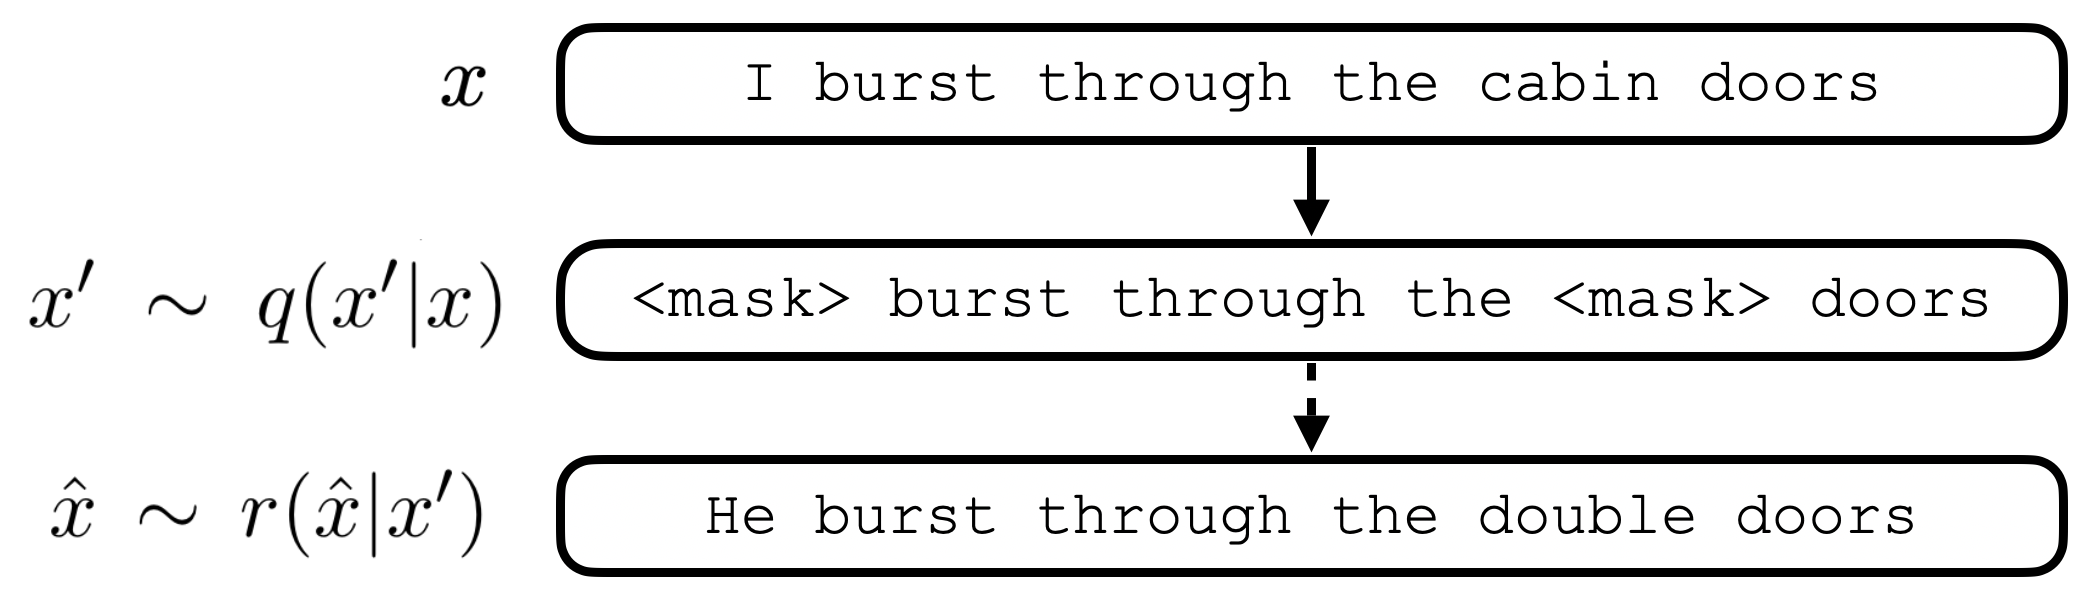
\includegraphics[scale=0.21]{img/bert_dae.png}
\caption{To sample from an MLM DAE, we apply the MLM corruption $q$ to the original sentence then reconstruct the corrupted sentence using our DAE $r$.}
\label{fig:dae_sampling}
\end{figure}

\subsection{Sampling from Denoising Autoencoders}
A denoising autoencoder (DAE) is an autoencoder trained to reconstruct a clean input $x$ from a stochastically corrupted one $x'\sim q(x'|x)$ by learning a conditional distribution $P_\theta (x| x')$ \citep{vincent2008extracting}.
We can sample from a DAE by successively corrupting and reconstructing an input using the following pseudo-Gibbs Markov chain: $x_t' \sim q(x'|x_{t-1})$, $x_t \sim P_\theta(x|x'_t).$
\comment{
\begin{align*}
    x_t' &\sim q(x'|x_{t-1})\\
    x_t &\sim P_\theta(x|x'_t) 
\end{align*}
}
As the number of training examples increases, the asymptotic distribution $\pi_n(x)$ of the generated samples approximate the true data-generating distribution $P(x)$ \citep{bengio2013generalized}.
This corruption-reconstruction process allows for sampling directly along the manifold that $P(x)$ concentrates on.

\subsection{Masked Language Models}
Recent advances in unsupervised representation learning for natural language have relied on pre-training models on a \textit{masked language modeling} (MLM) objective \citep{devlin2018, liu2019roberta}.
In the MLM objective, a percentage of the input tokens are randomly corrupted and the model is asked to reconstruct the original token given its left and right context in the corrupted sentence.
We use MLMs as DAEs \citep{lewis2019bart} to sample from the underlying natural language distribution by corrupting and reconstructing inputs (Figure \ref{fig:dae_sampling}).


\section{\sysname: Algorithm, Parallelism, and Work Partitioning}
\label{sec:algo}

We describe the \sysname algorithm, which includes several tweaks to \sysnameone
to reduce the number of non-matmul FLOPs.
We then describe how to parallelize the computation on different thread blocks
to make full use the GPU resources.
Finally we describe we partition the work between different warps within one
thread block to reduce the amount of shared memory access.
These improvements lead to 2-3$\times$ speedup as validated in~\cref{sec:experiments}.

\subsection{Algorithm}
\label{subsec:algo}

We tweak the algorithm from \sysnameone to reduce the number of non-matmul
FLOPs.
This is because modern GPUs have specialized compute units (e.g., Tensor Cores
on Nvidia GPUs) that makes matmul much faster.
As an example, the A100 GPU has a max theoretical throughput of 312 TFLOPs/s of
FP16/BF16 matmul, but only 19.5 TFLOPs/s of non-matmul FP32.
Another way to think about this is that each non-matmul FLOP is 16$\times$ more
expensive than a matmul FLOP.
To maintain high throughput (e.g., more than 50\% of the maximum theoretical
TFLOPs/s), we want to spend as much time on matmul FLOPs as possible.

\subsubsection{Forward pass}

We revisit the online softmax trick as shown in~\cref{subsec:flashv1} and make
two minor tweaks to reduce non-matmul FLOPs:
\begin{enumerate}
  \item We do not have to rescale both terms of the output update by $\diag(\ell^{(2)})^{-1}$:
  \begin{equation*}
    \vO^{(2)} = \diag(\ell^{(1)} / \ell^{(2)})^{-1} \vO^{(1)} + \diag(\ell^{(2)})^{-1} e^{\vS^{(2)} - m^{(2)}} \vV^{(2)}.
  \end{equation*}
  We can instead maintain an ``un-scaled'' version of $\vO^{(2)}$ and keep
  around the statistics $\ell^{(2)}$:
  \begin{equation*}
    \tilde{\vO}^{(2)} = \diag(\ell^{(1)})^{-1} \vO^{(1)} + e^{\vS^{(2)} - m^{(2)}} \vV^{(2)}.
  \end{equation*}
  Only at the every end of the loop do we scale the final
  $\tilde{\vO}^{(\mathrm{last})}$ by $\diag(\ell^{(\mathrm{last})})^{-1}$ to get
  the right output.

  \item We do not have to save both the max $m^{(j)}$ and the sum of
  exponentials $\ell^{(j)}$ for the backward pass. We only need to store the
  logsumexp $L^{(j)} = m^{(j)} + \log(\ell^{(j)})$.
\end{enumerate}

In the simple case of 2 blocks in~\cref{subsec:flashv1}, the online softmax
trick now becomes:
\begin{align*}
  m^{(1)} &= \mathrm{rowmax}(\vS^{(1)})  \in \mathbb{R}^{B_r}\\
  \ell^{(1)} &= \mathrm{rowsum}(e^{\vS^{(1)} - m^{(1)}}) \in \mathbb{R}^{B_r} \\
  \tilde{\vO^{(1)}} &= e^{\vS^{(1)} - m^{(1)}} \vV^{(1)} \in \mathbb{R}^{B_r \times d}\\
  m^{(2)} &= \max(m^{(1)}, \mathrm{rowmax}(\vS^{(2)})) = m \\
  \ell^{(2)} &= e^{m^{(1)} - m^{(2)}} \ell^{(1)} + \mathrm{rowsum}(e^{\vS^{(2)} - m^{(2)}}) = \mathrm{rowsum}(e^{\vS^{(1)} - m}) + \mathrm{rowsum}(e^{\vS^{(2)} - m}) = \ell \\
  \tilde{\vP}^{(2)} &= \diag(\ell^{(2)})^{-1} e^{\vS^{(2)} - m^{(2)}} \\
  \tilde{\vO}^{(2)} &= \diag(e^{m^{(1)} - m^{(2)}})^{-1} \tilde{\vO}^{(1)} + e^{\vS^{(2)} - m^{(2)}} \vV^{(2)} = e^{s^{(1)} - m} \vV^{(1)} + e^{s^{(2)} - m} \vV^{(2)} \\
  \vO^{(2)} &= \diag(\ell^{(2)})^{-1} \tilde{\vO}^{(2)} = \vO.
\end{align*}

We describe the full \sysname forward pass in~\cref{alg:flash2_fwd}.

\begin{algorithm}[H]
  % \algsetup{linenosize=\tiny}
  \caption{\small\label{alg:flash2_fwd}\sysname forward pass}
  \begin{algorithmic}[1]
    \REQUIRE Matrices $\vQ, \vK, \vV \in \mathbb{R}^{N \times d}$ in HBM, block sizes $B_c$, $B_r$.
    \STATE \label{alg:stream_attn_split_qkv} Divide $\vQ$ into $T_r = \left\lceil\frac{N}{B_r} \right\rceil$ blocks $\vQ_1, \dots, \vQ_{T_r}$ of size $B_r \times d$ each,
    and divide $\vK, \vV$ in to $T_c = \left\lceil \frac{N}{B_c} \right\rceil$ blocks $\vK_1, \dots, \vK_{T_c}$ and
    $\vV_1, \dots, \vV_{T_c}$, of size $B_c \times d$ each.
    \STATE Divide the output $\vO \in \mathbb{R}^{N \times d}$ into $T_r$ blocks $\vO_i, \dots, \vO_{T_r}$ of size
    $B_r \times d$ each, and divide the logsumexp $L$ into $T_r$ blocks $L_i, \dots, L_{T_r}$ of size
    $B_r$ each.
    \FOR{$1 \le i \le T_r$} \label{alg:stream_attn_outer_loop}
      \STATE \label{alg:stream_attn_load_q} Load $\vQ_i$ from HBM to on-chip SRAM.
      \STATE \label{alg:stream_attn_init} On chip, initialize $\vO_{i}^{(0)} = (0)_{B_r \times d} \in \mathbb{R}^{B_r \times d}, \ell_{i}^{(0)} = (0)_{B_r} \in \mathbb{R}^{B_r}, m_{i}^{(0)} = (-\infty)_{B_r} \in \mathbb{R}^{B_r}$.
      \FOR{$1 \le j \le T_c$}
        \STATE \label{alg:stream_attn_load_kv} Load $\vK_j, \vV_j$ from HBM to on-chip SRAM.
        \STATE \label{alg:stream_attn_qk} On chip, compute $\vS_{i}^{(j)} = \vQ_i \vK_j^T \in \mathbb{R}^{B_r \times B_c}$.
        \STATE \label{alg:stream_attn_statistics} On chip, compute
        $m_{i}^{(j)} = \mathrm{max}(m_{i}^{(j-1)}, \mathrm{rowmax}(\vS_{i}^{(j)})) \in \mathbb{R}^{B_r}$, $\tilde{\vP}_{i}^{(j)} = \exp(\vS_{i}^{(j)} - m_{i}^{(j)}) \in \mathbb{R}^{B_r \times B_c}$ (pointwise),
        $\ell_{i}^{(j)} = e^{m_{i}^{j-1} - m_{i}^{(j)}} \ell_{i}^{(j-1)} + \mathrm{row sum}(\tilde{\vP}_{i}^{(j)}) \in \mathbb{R}^{B_r}$.
        \STATE \label{alg:stream_attn_update} On chip, compute
        $\vO_{i}^{(j)} = \diag(e^{m_{i}^{(j-1)} - m_{i}^{(j)}})^{-1} \vO_{i}^{(j-1)} + \tilde{\vP}_{i}^{(j)} \vV_j$.
      \ENDFOR
      \STATE On chip, compute $\vO_{i} = \diag(\ell_{i}^{(T_c)})^{-1} \vO_{i}^{(T_c)}$.
      \STATE On chip, compute $L_{i} = m_{i}^{(T_c)} + \log(\ell_i^{(T_c)})$.
      \STATE Write $\vO_{i}$ to HBM as the $i$-th block of $\vO$.
      \STATE Write $L_{i}$ to HBM as the $i$-th block of $L$.
    \ENDFOR
    \STATE Return the output $\vO$ and the logsumexp $L$.
  \end{algorithmic}
\end{algorithm}

\paragraph{Causal masking.}

One common use case of attention is in auto-regressive language modeling, where
we need to apply a causal mask to the attention matrix $\vS$ (i.e., any entry
$\vS_{ij}$ with $j > i$ is set to $-\infty$).
\begin{enumerate}
  \item As \sysnameone and \sysname already operate by blocks, for any blocks
  where all the column indices are more than the row indices (approximately half
  of the blocks for large sequence length), we can skip the computation of that
  block.
  This leads to around 1.7-1.8$\times$ speedup compared to attention without the
  causal mask.
  \item We do not need to apply the causal mask for blocks whose row indices are
  guaranteed to be strictly less than the column indices. This means that for
  each row, we only need apply causal mask to 1 block (assuming square block).
\end{enumerate}

\paragraph{Correctness, runtime, and memory requirement.}
As with \sysnameone, \cref{alg:flash2_fwd} returns the correct output
$\vO = \softmax(\vQ\vK^\top)\vV$ (with no approximation), using $O(N^2d)$ FLOPs and
requires $O(N)$ additional memory beyond inputs and output (to store the
logsumexp $L$).
The proof is almost the same as the proof of
\citet[Theorem 1]{dao2022flashattention}, so we omit it here.

\subsubsection{Backward pass}

The backward pass of \sysname is almost the same as that of \sysnameone. We make
a minor tweak to only use the row-wise logsumexp $L$ instead of both the
row-wise max and row-wise sum of exponentials in the softmax.
We include the backward pass description in~\cref{alg:flash_bwd} for completeness.
\begin{algorithm}[h]
  \caption{\small\label{alg:flash_bwd}\sysname Backward Pass}
  \begin{algorithmic}[1]
    \REQUIRE Matrices $\vQ, \vK, \vV, \vO, \vdO \in \mathbb{R}^{N \times d}$ in HBM,
    vector $L \in \mathbb{R}^N$ in HBM, block sizes $B_c$, $B_r$.
    \STATE Divide $\vQ$ into $T_r = \left\lceil\frac{N}{B_r} \right\rceil$ blocks $\vQ_1, \dots, \vQ_{T_r}$ of size $B_r \times d$ each,
    and divide $\vK, \vV$ in to $T_c = \left\lceil \frac{N}{B_c} \right\rceil$ blocks $\vK_1, \dots, \vK_{T_c}$ and
    $\vV_1, \dots, \vV_{T_c}$, of size $B_c \times d$ each.
    \STATE Divide $\vO$ into $T_r$ blocks $\vO_i, \dots, \vO_{T_r}$ of size
    $B_r \times d$ each, divide $\vdO$ into $T_r$ blocks $\vdO_i, \dots, \vdO_{T_r}$
    of size $B_r \times d$ each, and divide $L$ into $T_r$ blocks $L_i, \dots, L_{T_r}$ of size
    $B_r$ each.
    \STATE Initialize $\vdQ = (0)_{N \times d}$ in HBM and divide it into $T_r$ blocks $\vdQ_1, \dots, \vdQ_{T_r}$ of size $B_r \times d$ each.
    Divide $\vdK, \vdV \in \mathbb{R}^{N \times d}$ in to $T_c$ blocks $\vdK_1, \dots, \vdK_{T_c}$ and
    $\vdV_1, \dots, \vdV_{T_c}$, of size $B_c \times d$ each.
    \STATE Compute $D = \mathrm{rowsum}(\vdO \circ \vO) \in \mathbb{R}^d$ (pointwise multiply), write
    $D$ to HBM and divide it into $T_r$ blocks $D_1, \dots, D_{T_r}$ of size
    $B_r$ each.
    \FOR{$1 \le j \le T_c$}
      \STATE Load $\vK_j, \vV_j$ from HBM to on-chip SRAM.
      \STATE Initialize $\vdK_j = (0)_{B_c \times d}, \vdV_j = (0)_{B_c \times d}$ on SRAM.
      \FOR{$1 \le i \le T_r$}
        \STATE Load $\vQ_i, \vO_i, \vdO_i, \vdQ_i, L_i, D_i$ from HBM to on-chip SRAM.
        \STATE On chip, compute $\vS_{i}^{(j)} = \vQ_i \vK_j^T \in \mathbb{R}^{B_r \times B_c}$.
        \STATE On chip, compute $\vP_{i}^{(j)} = \exp(\vS_{ij} - L_{i}) \in \mathbb{R}^{B_r \times B_c}$.
        \STATE On chip, compute
        $\vdV_j \leftarrow \vdV_j + (\vP_{i}^{(j)})^\top \vdO_i \in \mathbb{R}^{B_c \times d}$.
        \STATE On chip, compute
        $\vdP_{i}^{(j)} = \vdO_{i} \vV_j^\top \in \mathbb{R}^{B_r \times B_c}$.
        \STATE On chip, compute $\vdS_{i}^{(j)} = \vP_{i}^{(j)} \circ (\vdP_{i}^{(j)} - D_i) \in \mathbb{R}^{B_r \times B_c}$.
        \STATE Load $\vdQ_i$ from HBM to SRAM, then on chip, update
        $\vdQ_{i} \leftarrow \vdQ_i + \vdS_{i}^{(j)} \vK_j \in \mathbb{R}^{B_r \times d}$, and write
        back to HBM.
        \STATE On chip, compute $\vdK_{j} \leftarrow \vdK_j + {\vdS_{i}^{(j)}}^\top \vQ_i \in \mathbb{R}^{B_c \times d}$.
      \ENDFOR
      \STATE Write $\vdK_j, \vdV_j$ to HBM.
    \ENDFOR
    \STATE Return $\vdQ, \vdK, \vdV$.
  \end{algorithmic}
\end{algorithm}

\paragraph{Multi-query attention and grouped-query attention.}
Multi-query attention (MQA)~\citep{shazeer2019fast} and grouped-query attention
(GQA)~\citep{ainslie2023gqa} are variants of attention where multiple heads of
query attend to the same head of key and value, in order to reduce the size of
KV cache during inference.
Instead of having to duplicate the key and value heads for the computation, we
implicitly manipulate the indices into the head to perform the same computation.
In the backward pass, we need to sum the gradients $\vdK$ and $\vdV$ across
different heads that were implicitly duplicated.

\subsection{Parallelism}
\label{subsec:parallelism}

The first version of \sysnameone parallelizes over batch size and number of
heads.
We use 1 thread block to process one attention head, and there are overall
$\text{batch size} \cdot \text{number of heads}$ thread blocks.
Each thread block is scheduled to run on a streaming multiprocessor (SM), and
there are 108 of these SMs on an A100 GPU for example.
This scheduling is efficient when this number is large (say $\geq 80$), since we
can effectively use almost all of the compute resources on the GPU.

In the case of long sequences (which usually means small batch sizes or small
number of heads), to make better use of the multiprocessors on the GPU, we now
additionally parallelize over the sequence length dimension.
This results in significant speedup for this regime.


\paragraph{Forward pass.}
We see that the outer loop (over sequence length) is embarrassingly parallel,
and we schedule them on different thread blocks that do not need to communicate
with each other.
We also parallelize over the batch dimension and number of heads dimension, as
done in \sysnameone.
The increased parallelism over sequence length helps improve occupancy (fraction
of GPU resources being used) when the batch size and number of heads are small,
leading to speedup in this case.

These ideas of swapping the order of the loop (outer loop over row blocks and
inner loop over column blocks, instead of the other way round in the original
\sysnameone paper), as well as parallelizing over the sequence length dimension
were first suggested and implemented by Phil Tillet in the
Triton~\citep{tillet2019triton}
implementation.\footnote{\url{https://github.com/openai/triton/blob/main/python/tutorials/06-fused-attention.py}}

\paragraph{Backward pass.}
Notice that the only shared computation between different column blocks is in
update $\vdQ$ in \cref{alg:flash_bwd}, where we need to load $\vdQ_i$ from HBM
to SRAM, then on chip, update
$\vdQ_{i} \leftarrow \vdQ_i + \vdS_{i}^{(j)} \vK_j$, and write back to HBM.
We thus parallelize over the sequence length dimension as well, and schedule 1
thread block for each column block of the backward pass.
We use atomic adds to communicate between different thread blocks to update $\vdQ$.

We describe the parallelization scheme in \cref{fig:parallelism}.
\begin{figure}[ht]
  \centering
  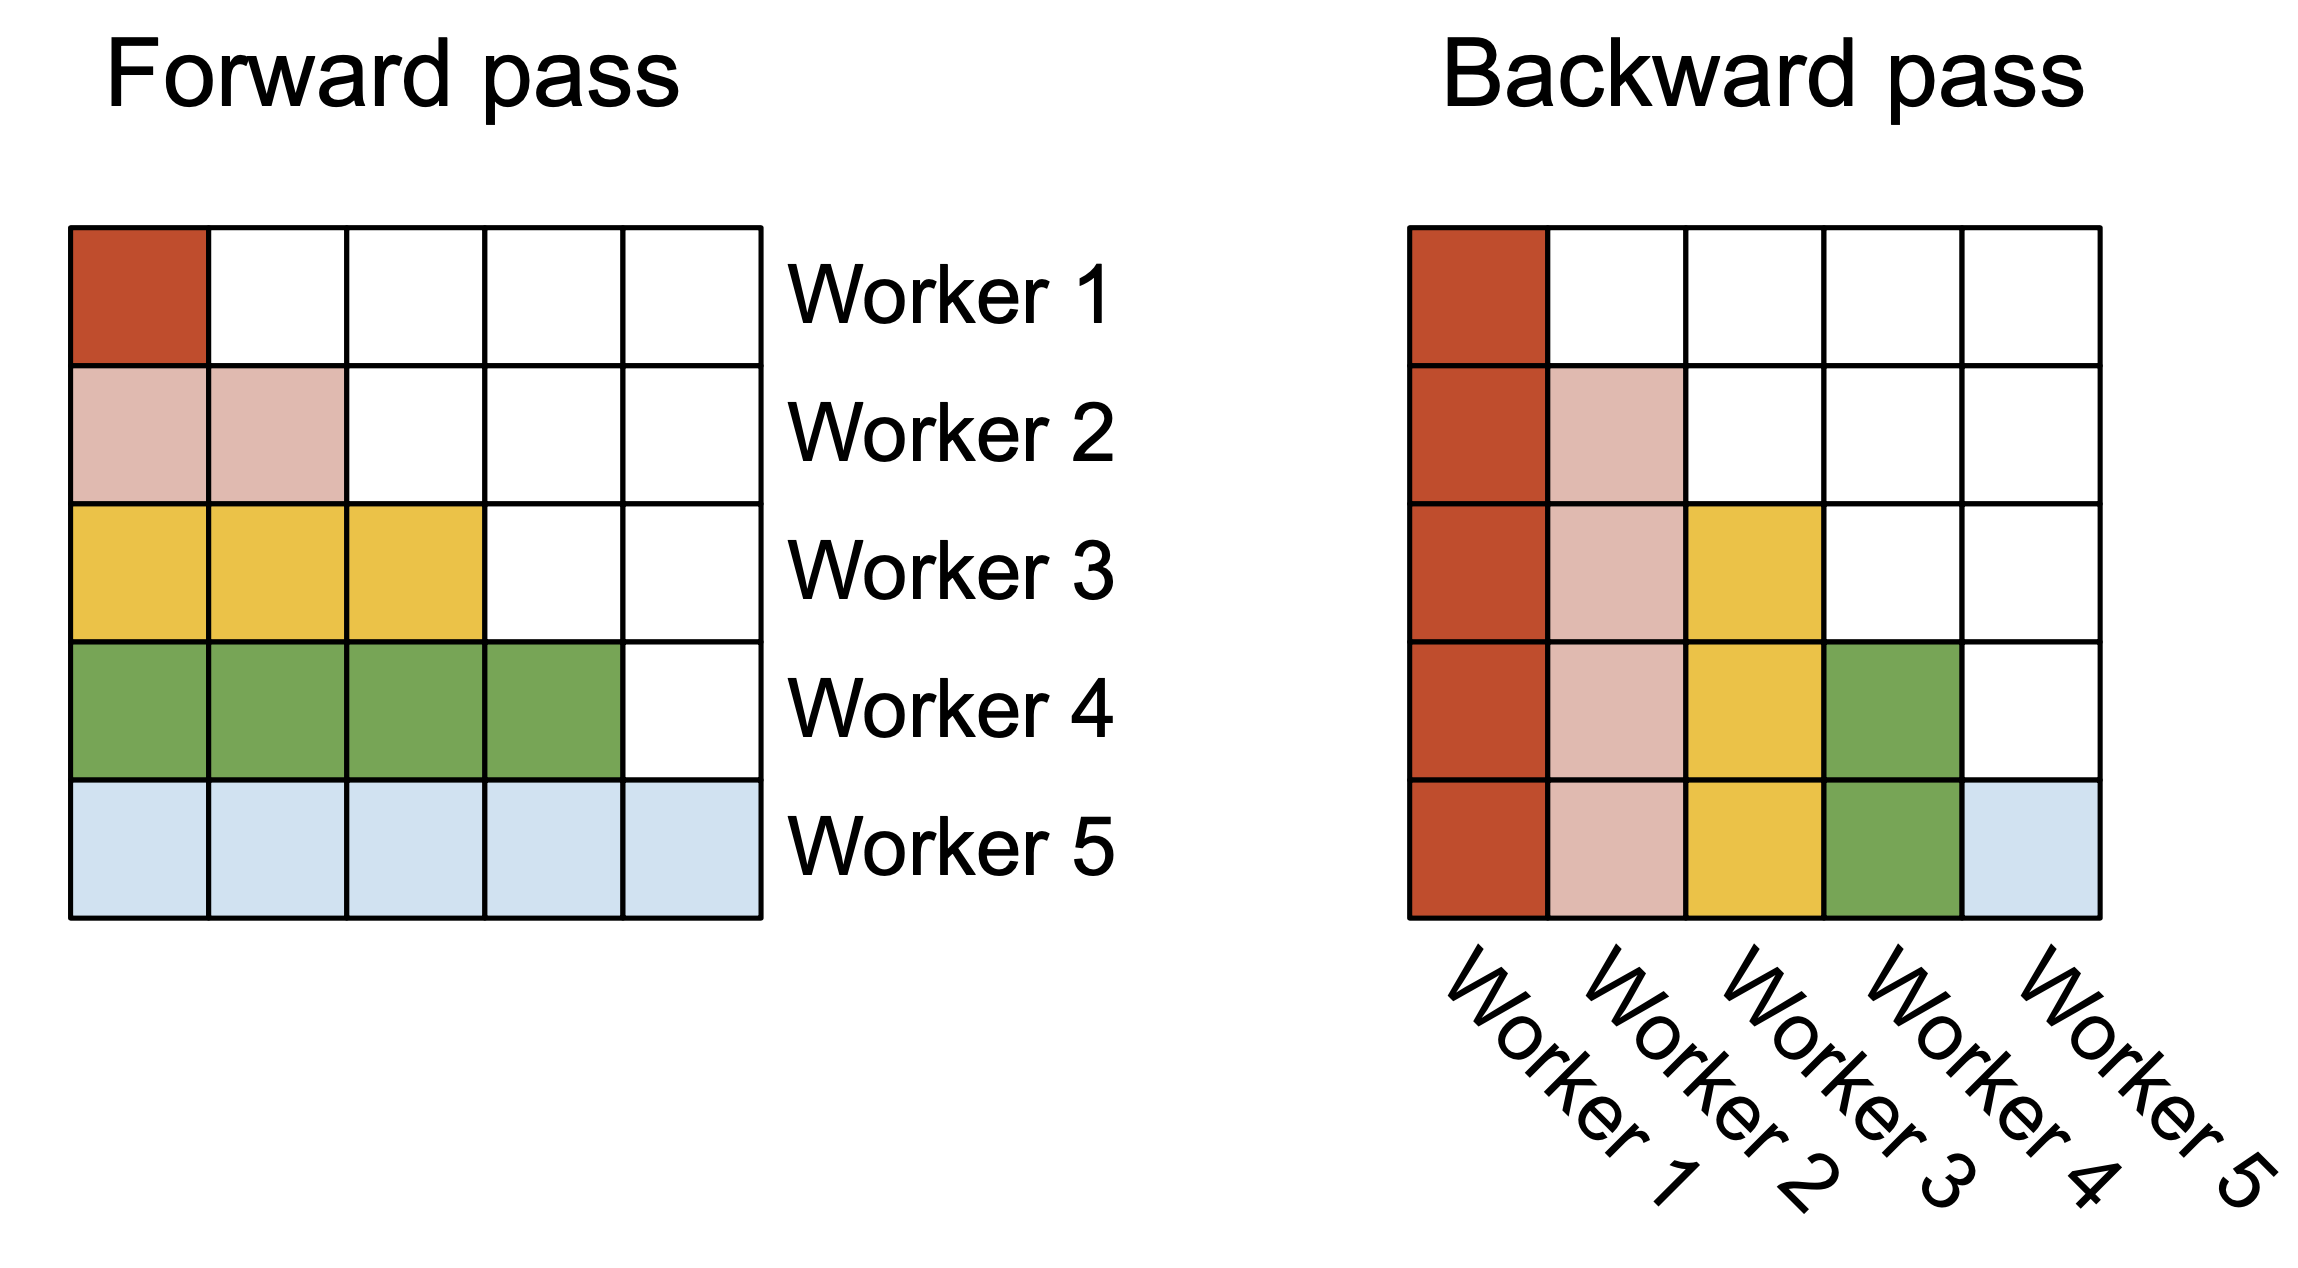
\includegraphics[width=0.95\linewidth]{figs/flashattention_fwd_bwd_parallel.png}
  \caption{\label{fig:parallelism}In the forward pass (left), we parallelize the
    workers (thread blocks) where each worker takes care of a block of rows of
    the attention matrix.
    In the backward pass (right), each worker takes care of a block of columns
    of the attention matrix.}
\end{figure}


\subsection{Work Partitioning Between Warps}
\label{subsec:work_partitioning}

As \cref{subsec:parallelism} describe how we schedule thread blocks, even within
each thread block, we also have to decide how to partition the work between
different warps.
We typically use 4 or 8 warps per thread block, and the partitioning is described
in \cref{fig:partitioning}.

\paragraph{Forward pass.}
For each block, \sysnameone splits $\vK$ and $\vV$ across 4 warps while keeping
$\vQ$ accessible by all warps.
Each warp multiplies to get a slice of $\vQ \vK^\top$, then they need to multiply
with a slice of $\vV$ and communicate to add up the result.
This is referred to as the ``split-K'' scheme.
However, this is inefficient since all warps need to write their intermediate
results out to shared memory, synchronize, then add up the intermediate results.
These shared memory reads/writes slow down the forward pass in \sysnameone.

In \sysname, we instead split $\vQ$ across 4 warps while keeping $\vK$ and $\vV$
accessible by all warps.
After each warp performs matrix multiply to get a slice of $\vQ \vK^\top$, they just need to
multiply with their shared slice of $\vV$ to get their corresponding
slice of the output.
There is no need for communication between warps.
The reduction in shared memory reads/writes yields speedup (\cref{sec:experiments}).

\begin{figure}[ht]
  \centering
  \begin{subfigure}{.53\textwidth}
    \centering
    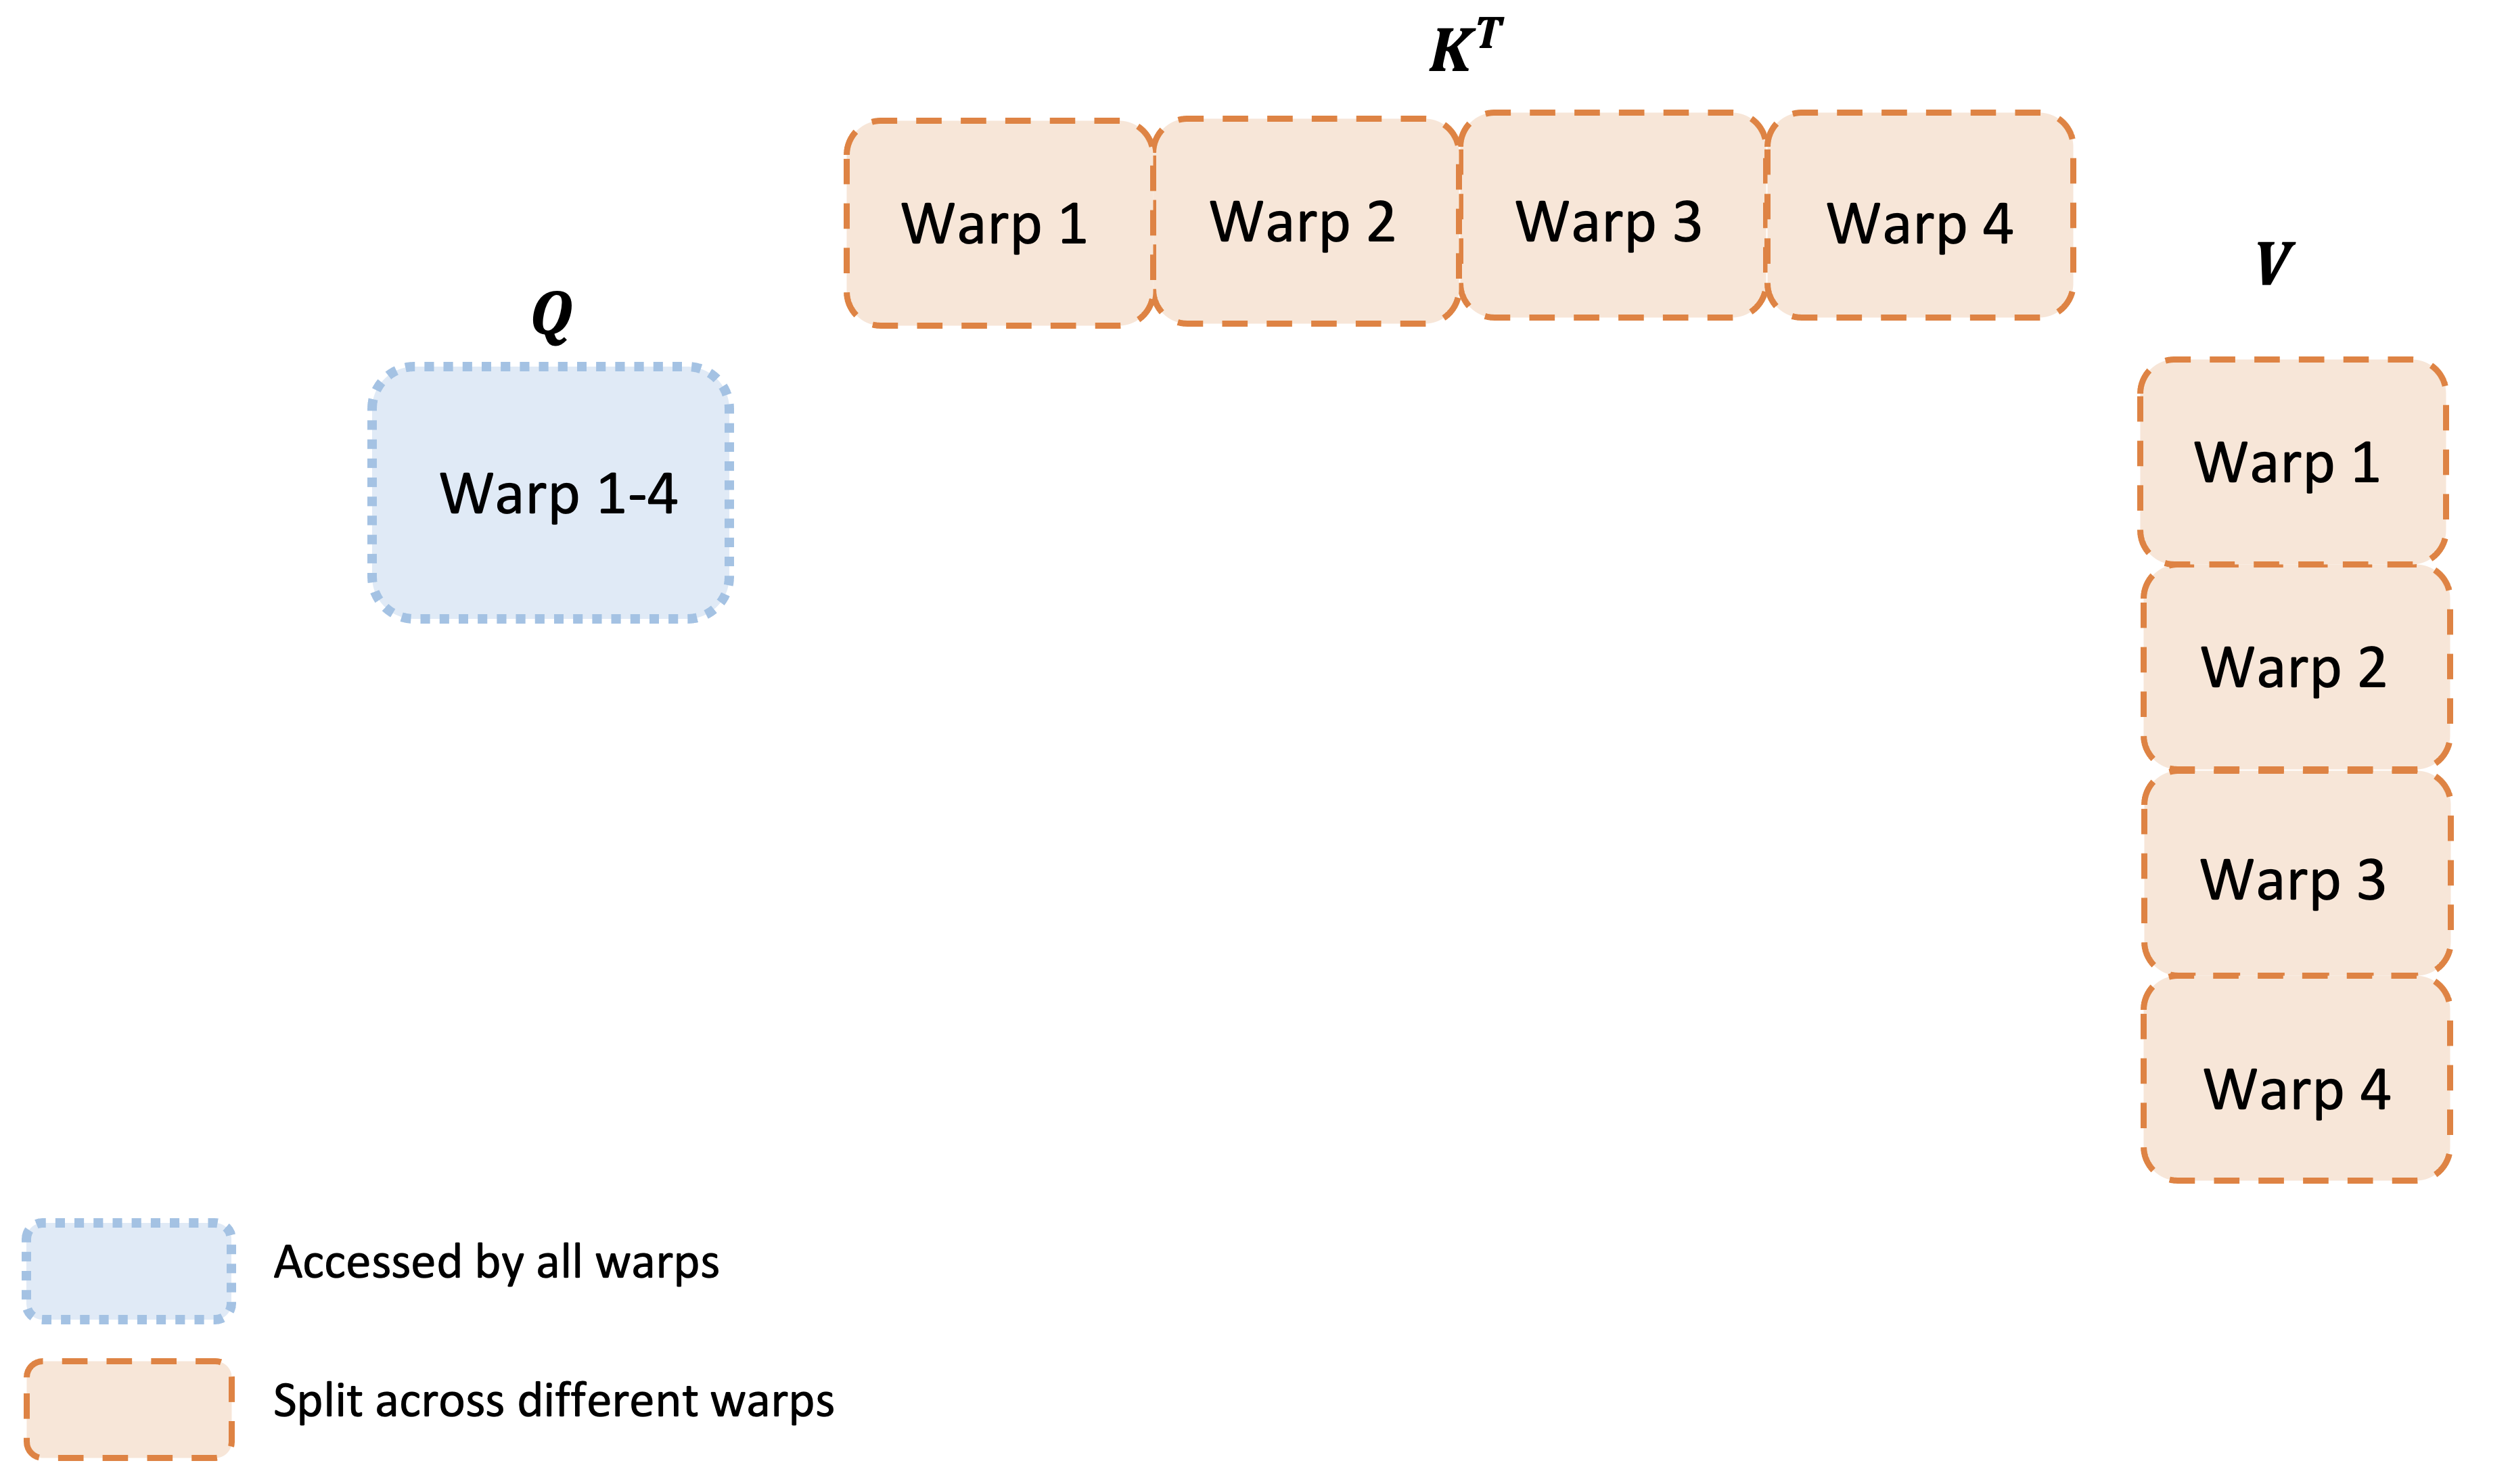
\includegraphics[width=.95\linewidth]{figs/flash_partitioning.png}
    \caption{\sysnameone}
  \end{subfigure}%
  \begin{subfigure}{.47\textwidth}
    \centering
    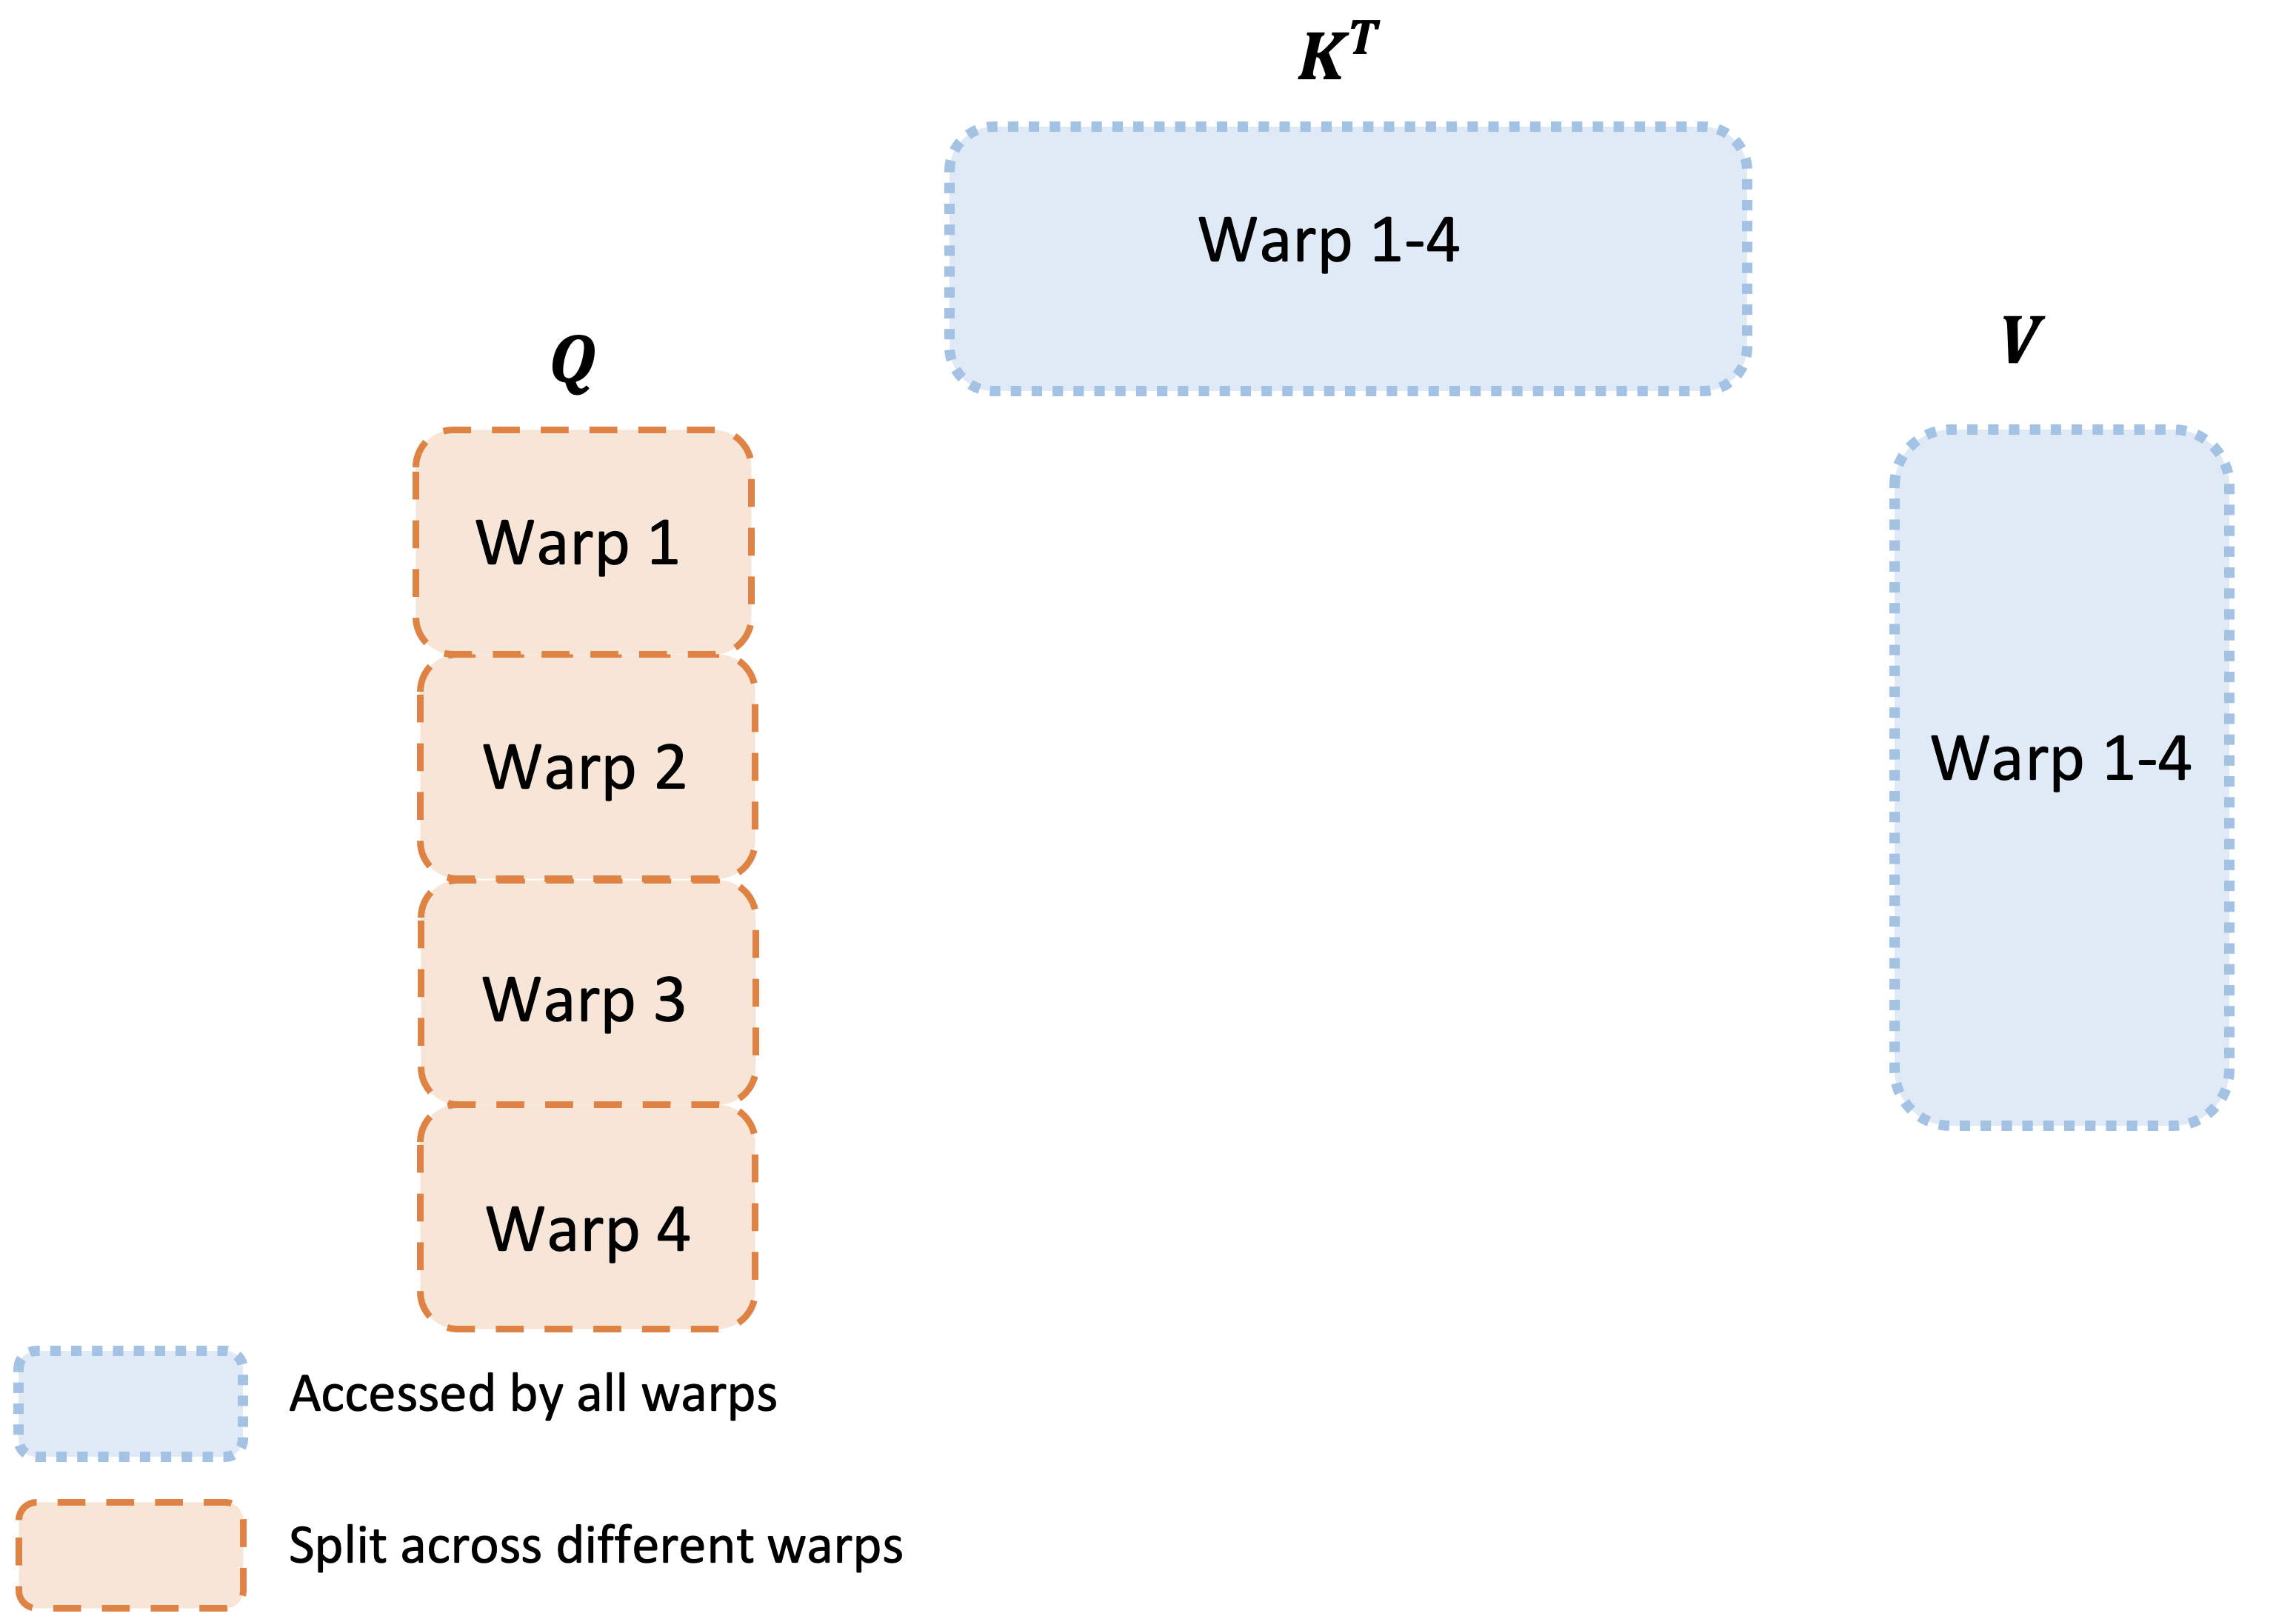
\includegraphics[width=.95\linewidth]{figs/flash2_partitioning.png}
    \caption{\sysname}
  \end{subfigure}
  \caption{Work partitioning between different warps in the forward pass}
  \label{fig:partitioning}
\end{figure}

\paragraph{Backward pass.}
Similarly for the backward pass, we choose to partition the warps to avoid the
``split-K'' scheme.
However, it still requires some synchronization due to the more complicated
dependency between all the different inputs and gradients
$\vQ, \vK, \vV, \vO, \vdO, \vdQ, \vdK, \vdV$.
Nevertheless, avoiding ``split-K'' reduces shared memory reads/writes and again
yields speedup (\cref{sec:experiments}).

\paragraph{Tuning block sizes}
Increasing block sizes generally reduces shared memory loads/stores, but
increases the number of registers required and the total amount of shared
memory.
Past a certain block size, register spilling causes significant slowdown, or the
amount of shared memory required is larger than what the GPU has available, and
the kernel cannot run at all.
Typically we choose blocks of size $\{64, 128\} \times \{64, 128\}$, depending on the
head dimension $d$ and the device shared memory size.

We manually tune for each head dimensions since there are essentially only 4
choices for block sizes, but this could benefit from auto-tuning to avoid this
manual labor.
We leave this to future work.

\section{Experiments}
\label{sec:experiments}

We validate our approach empirically, showing that our Monarch matrix parametrization achieves a favorable efficiency--accuracy tradeoff compared to baselines on a wide range of domains (text, images, PDEs, MRI), in three settings (E2E training, S2D training, and D2S fine-tuning):
\begin{itemize}[leftmargin=*,nosep,nolistsep,noitemsep]
\item
In \cref{subsec:benchmark_tasks}, on image classification and language modeling benchmarks, such as ViT / MLP Mixer on ImageNet and GPT-2 on Wikitext-103, Monarch is 2$\times$ faster to train than dense models, while achieving the same accuracy / perplexity. In \cref{subsec:pde_mri}, in scientific and medical domains where special transforms (Fourier) are common, Monarch outperforms Fourier transform based methods on PDE solving, with up to 40\% lower error, and on MRI reconstruction attains up to 15\% higher pSNR and 3.8\% higher SSIM.
\item In \cref{subsec:pde_mri}, we show that on the large OpenWebText dataset, reverse sparsification (training with Monarch weight matrices for most of the time, then transitioning to dense weight matrices) speeds up the pretraining of GPT-2 models by 2$\times$ compared to the dense model, with no loss in upstream or downstream quality.
Moreover, reverse sparsification speeds up BERT pretraining by 23\% even compared to the implementation from Nvidia that set the MLPerf~\citep{mattson2020mlperf} 1.1 record.
\item In \cref{subsec:finetuning}, as a proof of concept, we demonstrate that our Monarch approximation algorithm can improve fine-tuning efficiency for pretrained models. We show that compressing BERT to a Monarch matrix model performs comparably to a finetuned dense model on GLUE, with 2$\times$ fewer parameters and 1.7$\times$ faster finetuning speed.
\end{itemize}

\subsection{End-to-End Training}
\label{subsec:e2e_training}
\subsubsection{Benchmark Tasks: Image Classification, Language Modeling}
\label{subsec:benchmark_tasks}

We show that replacing dense matrices with Monarch matrices in ViT, MLP-Mixer, and
GPT-2 can speed up training by up to 2$\times$ without sacrificing model quality in~\cref{table:pretrain,table:gpt_pretrain}.

\textbf{Setup.} We use the popular vision benchmark, ImageNet~\citep{deng2009imagenet}. We choose recent popular Vision Transformer~\citep{dosovitskiy2020image}, and MLP-Mixer~\citep{tolstikhin2021mlp} as representative base dense models.
For language modeling, we evaluate GPT-2~\citep{radford2019language} on WikiText-103~\citep{merity2016pointer}.

\begin{table}[h]
  \small
  \centering
  \vspace{-2mm}
  \caption{\label{table:pretrain}The performance of Monarch matrices and ViT / MLP-Mixer on ImageNet, including the number of parameters and FLOPs. We measure the Top-1 accuracy and the training time speedup compared to the corresponding dense model. %
  \vspace{2mm}
  }
  \iftoggle{arxiv}{}{
  \resizebox{\linewidth}{!}
  }
  {
  \setlength{\tabcolsep}{3pt}
  \vspace{3em}
  \begin{tabular}{@{}c||ccccccc@{}}
  \specialrule{.15em}{.05em}{.05em}
    Model&\multicolumn{1}{c}{ImageNet acc.}&\multicolumn{1}{c}{Speedup} &\multicolumn{1}{c}{Params} & \multicolumn{1}{c}{FLOPs} \\
    \specialrule{.15em}{.05em}{.05em}
    Mixer-S/16& 74.0& - & 18.5M & 3.8G \\
    Monarch-Mixer-S/16& 73.7& 1.7$\times$ & 7.0M & 1.5G \\
    Mixer-B/16& 77.7& - & 59.9M & 12.6G \\
    Monarch-Mixer-B/16& 77.8& 1.9$\times$ & 20.9M & 5.0G \\
    \specialrule{.15em}{.05em}{.05em}
    ViT-S/16& 79.4 & - & 48.8M & 9.9G \\
    Monarch-ViT-S/16& 79.1 & 1.9$\times$ & 19.6M & 3.9G \\
    ViT-B/16& 78.5 & - & 86.6M  & 17.6G \\
    Monarch-ViT-B/16& 78.9 & 2.0$\times$ & 33.0M & 5.9G \\
    \specialrule{.15em}{.05em}{.05em}
  \end{tabular}
  }
\end{table}

\begin{table}[h]
  \small
  \centering
  \vspace{-3mm}
  \caption{\label{table:gpt_pretrain} Performance of Monarch matrices and GPT-2-Small/Medium on WikiText-103, including the \# of parameters and FLOPs. Monarch achieves similar perplexity (ppl) but 2.0$\times$ faster.}
  \vspace{1mm}
  \iftoggle{arxiv}{}{
    \resizebox{0.95\linewidth}{!}
  }
  {
\setlength{\tabcolsep}{5pt}
\begin{tabular}{c||cccc}
\specialrule{.15em}{.05em}{.05em}
\multirow{1}{*}{{ Model} } & \multicolumn{1}{c}{\multirow{1}{*}{PPL}}
                              & \multicolumn{1}{c}{\multirow{1}{*}{Speedup}}
                              & \multicolumn{1}{c}{\multirow{1}{*}{Params}}
                              & \multicolumn{1}{c}{\multirow{1}{*}{FLOPs}}\\
\specialrule{.15em}{.05em}{.05em}
GPT-2-Small &  20.6 & - & 124M& 106G\\
Monarch-GPT-2-Small& 20.7  & 1.8$\times$ &72M & 51G\\
\specialrule{.15em}{.05em}{.05em}
GPT-2-Medium &  20.9 & - & 355M& 361G\\
Monarch-GPT-2-Medium& 20.3  & 2.0$\times$ &165M & 166G\\
\specialrule{.15em}{.05em}{.05em}
\end{tabular}
}
\vspace{-2mm}
\end{table}


\subsubsection{PDE solving and multi-coil MRI reconstruction}
\label{subsec:pde_mri}

Many scientific or medical imaging tasks rely on specialized transforms such as the
Fourier transform.
We show that replacing the fixed Fourier transform with the more expressive
Monarch matrices yields higher model quality (lower reconstruction error) with
comparable model speed.

\textbf{Solving PDEs with Monarch Neural Operators.}
We follow the experimental setting in FNO~\citep{li2020fourier} and apply a Monarch--based neural operator to the task of solving the Navier--Stokes PDE. Compared to baseline U-Nets~\citep{ronneberger2015u}, TF-Nets~\citep{wang2020towards}, ResNets~\citep{he2016deep} and FNOs~\cite{li2020fourier}, neural operators based on Monarch improve solution accuracy across spatial resolutions by up to $40\%$ (Table \ref{table:pde}).  





\paragraph{Non-periodic boundary conditions.} Traditional spectral methods based on Fourier transform work best with periodic boundary conditions and forcing terms. However, PDEs of practical interest often exhibit non--periodic or even unknown boundary conditions. Monarch operators are not constrained to the Fourier transform and can thus still learn the solution operator with excellent accuracy.

\begin{table}[h!] 
\scriptsize
\vspace{-4mm}
\caption{\label{table:pde}Benchmarks on Navier-Stokes (fixing resolution 64 × 64 for both training and testing).
Decreasing the viscosity coefficient $\nu$ makes the dynamics more chaotic.
}
\vspace{1mm}
\centering
\iftoggle{arxiv}{}{
  \resizebox{0.9\linewidth}{!}
}
{
\renewcommand{\arraystretch}{1}
\begin{tabular}{ c||ccc }
\specialrule{.15em}{.05em}{.05em}
Model & $v = 10^{-3}$  &  $v = 10^{-4}$ & $v = 10^{-5}$\\
\specialrule{.15em}{.05em}{.05em}
U-Net & 0.025  & 0.205  &   0.198\\
TF-Net  & 0.023  & 0.225 &  0.227 \\
ResNet & 0.070 &  0.287 &  0.275 \\
FNO & 0.017  & 0.178 & 0.155\\
Monarch-NO & \textbf{0.010} & \textbf{0.145} & \textbf{0.136} \\
\specialrule{.15em}{.05em}{.05em}
\end{tabular}
}
\textbf{\vspace{-3mm}}
\end{table}

\textbf{Accelerated MRI Reconstruction.} We characterize the utility of Monarch-based FFT operations for accelerated MRI reconstruction, a task which requires methods with both structured Fourier operators and dealiasing properties to recover high quality images. On the clinically-acquired 3D MRI SKM-TEA dataset \citep{desai2021skm}, Monarch-SENSE (mSENSE) enhances image quality by over 1.5dB pSNR and 2.5\% SSIM compared to zero-filled SENSE and up to 4.4dB and 3.8\% SSIM compared to U-Net baselines in data-limited settings. Setup details are available in~\cref{sec:experiment_details_mri}.

\paragraph{Expressive FFT.} By definition, standard IFFT in zero-filled SENSE cannot dealias the signal, resulting in artifacts in the reconstructed image. mSENSE replaces the inverse FFT (IFFT) operation in standard SENSE with learnable Monarch matrices. Thus, mSENSE preserves the structure of the Fourier transform while learning to reweight frequencies to suppress aliasing artifacts. Across multiple accelerations, mSENSE achieved up to +1.5dB and 2.5\% improvement in peak signal-to-noise ratio (pSNR) and structural similarity (SSIM), respectively (Table~\ref{table:mri}).

\paragraph{Data Efficiency.} While CNNs have shown promise for MRI reconstruction tasks, training these networks requires extensive amounts of labeled data to avoid overfitting. However, large data corpora are difficult to acquire in practice. mSENSE can be trained efficiently with limited supervised examples. In few shot settings, mSENSE can outperform U-Net by +4.4dB ($\approx$15\%) and 3.8\% SSIM (Table~\ref{table:mri-data-limited}). 







\begin{table}[h!] 
\scriptsize
\vspace{-3mm}
\caption{\label{table:mri}Mean $\pm$ standard error of the mean of conventional and Monarch-SENSE (mSENSE) on dual-echo (E1,E2) MRI reconstruction at multiple acceleration factors (Acc.).
}
\vspace{1mm}
\centering
\iftoggle{arxiv}{}{
  \resizebox{\linewidth}{!}
}
{
\renewcommand{\arraystretch}{1.2}
\begin{tabular}{c||ccccc}
\specialrule{.15em}{.05em}{.05em}
  & & \multicolumn{2}{c}{pSNR (dB) ($\uparrow$)} & \multicolumn{2}{c}{SSIM ($\uparrow$)} \\
  Acc. & Model &             E1 &             E2 &                E1 &                E2 \\
\specialrule{.15em}{.05em}{.05em}
\multirow{2}{*}{2} & SENSE &  32.8$\pm$0.2 &  35.4$\pm$0.2 &  0.871$\pm$0.003 &  0.865$\pm$0.003 \\
  & mSENSE &  \textbf{34.3$\pm$0.2} &  \textbf{36.6$\pm$0.2} &  \textbf{0.886$\pm$0.002} &  \textbf{0.882$\pm$0.003} \\
\specialrule{.15em}{.05em}{.05em}
\multirow{2}{*}{3} & SENSE &  30.9$\pm$0.2 &  33.5$\pm$0.2 &  0.819$\pm$0.004 &  0.795$\pm$0.004 \\
  & mSENSE &  \textbf{32.3$\pm$0.2} &  \textbf{34.6$\pm$0.2} &  \textbf{0.843$\pm$0.003} &  \textbf{0.820$\pm$0.004} \\
\specialrule{.15em}{.05em}{.05em}
\multirow{2}{*}{4} & SENSE &  30.1$\pm$0.2 &  32.8$\pm$0.2 &  0.789$\pm$0.004 &  0.753$\pm$0.005 \\
  & mSENSE &  \textbf{31.2$\pm$0.2} &  \textbf{33.5$\pm$0.2} &  \textbf{0.812$\pm$0.003} &  \textbf{0.767$\pm$0.005} \\
\specialrule{.15em}{.05em}{.05em}
\end{tabular}
}
\end{table}

\begin{table}[h!] 
\scriptsize
\vspace{-5mm}
\caption{\label{table:mri-data-limited}Impact of number of training examples ($N$) on dual-echo MRI reconstruction at 2x acceleration.
}
\vspace{1mm}
\centering
\iftoggle{arxiv}{}{
  \resizebox{\linewidth}{!}
}
{
\renewcommand{\arraystretch}{1.2}
\begin{tabular}{c||ccccc}
\specialrule{.15em}{.05em}{.05em}
  &  & \multicolumn{2}{c}{pSNR (dB) ($\uparrow$)} & \multicolumn{2}{c}{SSIM ($\uparrow$)} \\
  $N$ & Model &            E1 &            E2 &               E1 &               E2 \\
\specialrule{.15em}{.05em}{.05em}
N/A & SENSE &  32.8$\pm$0.2 &  35.4$\pm$0.2 &  0.871$\pm$0.003 &  0.865$\pm$0.003 \\
\specialrule{.15em}{.05em}{.05em}
\multirow{2}{*}{1} & U-Net &  29.4$\pm$0.2 &  34.4$\pm$0.3 &  0.848$\pm$0.004 &  0.857$\pm$0.004 \\
  & mSENSE &  \textbf{33.8$\pm$0.2} &  \textbf{36.0$\pm$0.2} &  \textbf{0.886$\pm$0.003} &  \textbf{0.867$\pm$0.003} \\
\specialrule{.15em}{.05em}{.05em}
\multirow{2}{*}{2} & U-Net &  29.9$\pm$0.3 &  35.1$\pm$0.3 &  0.858$\pm$0.003 &  0.871$\pm$0.003 \\
  & mSENSE &  \textbf{34.0$\pm$0.2} &  \textbf{36.4$\pm$0.2} &  \textbf{0.883$\pm$0.002} &  \textbf{0.877$\pm$0.003} \\
\specialrule{.15em}{.05em}{.05em}
\multirow{2}{*}{3} & U-Net &  31.0$\pm$0.3 &  35.2$\pm$0.3 &  0.866$\pm$0.003 &  0.867$\pm$0.004 \\
  & mSENSE &  \textbf{33.9$\pm$0.2} & \textbf{ 36.5$\pm$0.2} &  \textbf{0.882$\pm$0.002} & \textbf{0.878$\pm$0.003} \\
\specialrule{.15em}{.05em}{.05em}
\multirow{2}{*}{5} & U-Net &  31.4$\pm$0.3 &  35.6$\pm$0.2 &  0.877$\pm$0.002 &  0.870$\pm$0.003 \\
  & mSENSE &  \textbf{33.9$\pm$0.2} &  \textbf{36.5$\pm$0.2} &  \textbf{0.881$\pm$0.002} &  \textbf{0.877$\pm$0.003} \\
\specialrule{.15em}{.05em}{.05em}
\end{tabular}
}
\end{table}




\subsection{Sparse-to-Dense Training (reverse sparsification)}
\label{subsec:s2d_training}
\paragraph{GPT-2 pretraining.}
On the large OpenWebtext dataset~\citep{Gokaslan2019OpenWeb}, we train a GPT-2 model with Monarch weight
matrices for 90\% of the training iterations, then relax the constraint on the
weight matrices and train them as dense matrices for the remaining 10\% of the
iterations.
We call this technique ``reverse sparsification.''
Previous sparse training techniques often don't speed up training, whereas our
hardware-efficient Monarch matrices do.
Therefore we can use them as an intermediate step to pretrain a large language
model (GPT-2) in 2$\times$ less time. We also evaluate its downstream quality on zero-shot generation from~\citep{eval-harness} and classification tasks from~\citep{zhao2021calibrate}, achieving comparable performance to the dense counterparts (\cref{table:gpt_finetune}). 

\begin{table}[h]
  \small
  \centering
  \vspace{-3mm}
  \caption{\label{table:gpt_finetune}The performance (accuracy) of GPT-2-medium trained with Monarch reverse sparsification and with conventional dense training on text classification benchmarks.}
  \setlength{\tabcolsep}{5pt}
  \vspace{1em}
  \iftoggle{arxiv}{}{
    \resizebox{\linewidth}{!}
  }
  {
  \begin{tabular}{@{}c||ccc@{}}
    \specialrule{.15em}{.05em}{.05em}
    Model&\multicolumn{1}{c}{OpenWebText (ppl)}&\multicolumn{1}{c}{Speedup}& \multicolumn{1}{c}{Classification (avg acc)} \\
    \specialrule{.15em}{.05em}{.05em}
    GPT-2m& 18.0 & - & 38.9 \\
    Monarch-GPT-2m& 18.0 & 2$\times$ & 38.8 \\
    \specialrule{.15em}{.05em}{.05em}
  \end{tabular}
  }
  \vspace{-3mm}
\end{table}


In \cref{fig:reverse_sparsification_bar}, we show the training time of the dense GPT-2 model, along with
the Monarch GPT-2 model.
After training the Monarch model for 90\% of the time, in the
last 10\% of the training steps, by transitioning to dense weight matrices, the model is able to reach the same 
performance of another model that was trained with dense weight matrices from
scratch.
By training with Monarch matrices for 90\% of the time, we reduce the total training time by 2$\times$.

\paragraph{BERT pretraining.}
On the Wikipedia + BookCorpus datasets~\citep{zhu2015aligning}, we train a BERT-large model with Monarch weight matrices for 70\% of the time and transition to dense weight matrices for the remaining 30\% of the time, which yields the same pretraining loss as conventional dense training.
In \cref{table:bert_speed}, we compare the total training time to several baseline implementations: the widely-used implementation from HuggingFace~\citep{wolf-etal-2020-transformers}, the more optimized implementation from Megatron~\citep{shoeybi2019megatron}, and the most optimized implementation we know of from Nvidia that was used to set MLPerf 1.1 training speed record. Our method is 3.5x faster than HuggingFace and 23\% faster than Nvidia's MLPerf 1.1 implementation\footnote{Our result is not an official MLPerf submission. We train BERT for both phase 1 (sequence length 128) and phase 2 (sequence length 512) according to the standard BERT training recipe\cite{devlin2018bert}, while MLPerf only measures training time for phase 2.}.
Experiment details are in~\cref{subsec:bert_details}.

\begin{table}[h]
  \small
  \centering
  \caption{\label{table:bert_speed}The total training time of BERT-large trained with Monarch reverse sparsification and with conventional dense training on 8 A100-40GB GPUs (DGX A100). Training consists of two phases, phase 1 with sequence length 128 and phase 2 with sequence length 512. Monarch training is 3.5x faster than HuggingFace and 23\% faster than Nvidia's MLPerf 1.1 implementation.}
  \vspace{1em}
  \iftoggle{arxiv}{}{
    \resizebox{\linewidth}{!}
  }
  {
    \begin{tabular}{@{}c||c@{}}
      Implementation & Training time (h)  \\ \hline
      HuggingFace &  84.5 \\
      MegaTron & 52.5 \\
      Nvidia MLPerf 1.1 & 30.2 \\
      Nvidia MLPerf 1.1 + DeepSpeed & 29.3 \\
      Monarch (ours) & \textbf{23.8} \\
    \end{tabular}
  }
  \vspace{-3mm}
\end{table}

\subsection{Dense-to-Sparse Fine-tuning}
\label{subsec:finetuning}

\begin{figure}[t]
  \centering
  \vspace{-3mm}
  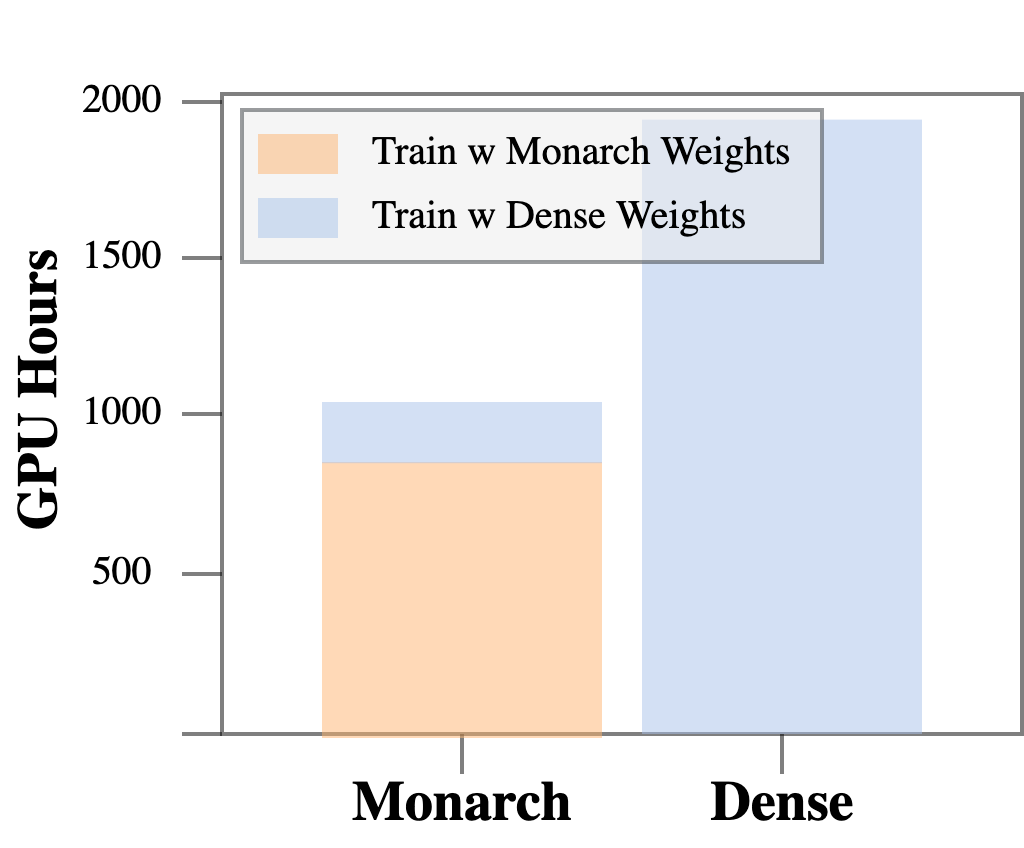
\includegraphics[width=.3\textwidth]{figures/rv_bar_temp.png}
  \vspace{-3mm}
  \caption{\label{fig:reverse_sparsification_bar}Time required (in A100 GPU hours) to reach the same perplexity (18.0)
    for GPT-2-small on OpenWebText.
    With ``reverse sparsification'', Monarch can speed up
    GPT-2 training by 2$\times$.\vspace{-1em}}
\end{figure}

We show that our Monarch approximation algorithm allows us to efficiently use
pretrained models, such as speeding up BERT finetuning on GLUE.

\paragraph{BERT finetuning.}
We take the BERT pretrained weights, approximate them with Monarch matrices,
and finetune the resulting model on the 9 GLUE tasks.
The results in \cref{table:bert_glue} shows that we obtain a Monarch finetuned
model with similar quality to the dense BERT model, but with 1.7$\times$ faster
finetuning speed.
This serves as a proof of concept, and we expect further speedup if additional model compression techniques are applied (e.g., quantization, kernel fusion).




\begin{table}[h]
  \small
  \centering
  \vspace{-5mm}
  \caption{\label{table:bert_glue}The performance of Monarch matrices in
    finetuning BERT on GLUE.}
  \setlength{\tabcolsep}{5pt}
  \vspace{1em}
  \iftoggle{arxiv}{}{
    \resizebox{\linewidth}{!}
  }
  {
  \begin{tabular}{@{}c||ccccccc@{}}
  \specialrule{.15em}{.05em}{.05em}
    Model&\multicolumn{1}{c}{GLUE (avg)}&\multicolumn{1}{c}{Speedup} &\multicolumn{1}{c}{Params} & \multicolumn{1}{c}{FLOPs} \\
    \specialrule{.15em}{.05em}{.05em}
    BERT-base & 78.6& - & 109M & 11.2G \\
    Monarch-BERT-base& 78.3& 1.5$\times$ & 55M & 6.2G  \\
    BERT-large & 80.4 & - & 335M & 39.5G \\
    Monarch-BERT-large & 79.6 & 1.7$\times$ & 144M & 14.6G  \\
    \specialrule{.15em}{.05em}{.05em}
  \end{tabular}
  }
  \vspace{-3mm}
\end{table}





We explored LLMs and their alignment with neural responses during language processing, uncovering several key findings. Firstly, we observed a clear correlation between the language task performance of LLMs and their accuracy in predicting neural responses in the auditory cortex, with higher-performing models exhibiting greater functional alignment with the speech cortex. Secondly, we showed that the models with higher performance on benchmark tasks achieved peak predictive accuracy in earlier layers. In contrast, lower-performing models exhibited a delayed representation, necessitating deeper layers to approach similar levels of brain prediction accuracy. Finally, our study highlights the crucial role of contextual information in both LLMs and brain processing, where the contextual window's size significantly influenced the difference between better and worse models, with the availability of long-range contextual information driving the high-performing LLMs closer to the brain's hierarchical pathway. These findings uncover fundamental principles in language processing, highlighting the critical role of hierarchical structure and contextual dependencies in language which give rise to convergent processing strategies in both artificial and biological systems. 

\subsection{Hierarchical Processing and Inter-Model Comparisons}
We found that better-performing LLMs exhibit a more brain-like hierarchy of layers, offering new insights into their language processing. While previous studies have revealed similarities in the hierarchical stages found in the brain and deep neural networks for linguistic \cite{caucheteux2023evidence, caucheteux2022brains, kumar2022reconstructing}, acoustic \cite{giordano2023intermediate, tuckute2023many}, visual \cite{kriegeskorte2015deep, cichy2016comparison, sexton2022reassessing}, and imagined stimuli \cite{horikawa2017hierarchical}, a distinct approach in our study is the inter-model comparison within a consistent architectural framework. In related work analyzing deep neural networks for vision tasks, recent evidence \cite{nonaka2021brain} has shown that better performance can create a less brain-like progression of feature extraction in models when compared to the visual cortex, suggesting that the complex architectures of high-performing image processing networks have steered them away from neural alignment. By examining LLMs based on a single architecture, the stacked transformer decoder \cite{vaswani2017attention}, we uncover differences in their alignment with the brain's hierarchical stages during language comprehension. Transformer language models use contextual features to encode linguistic, syntactic, and positional structures \cite{o2021context, clark2019does}, and increasingly high-level and context-specific features arise throughout a model’s layers \cite{ethayarajh2019contextual, tenney2019bert}. This may be partly because later layers bind linguistic structures over longer contexts \cite{skrill2023large}. The crucial observation that such models display brain-like hierarchies resonates with neurobiological findings of hierarchical organization in the auditory and language-related cortex \cite{hickok2007cortical, sharpee2011hierarchical, sheng2019cortical, ding2017characterizing, hasson2008hierarchy, lerner2011topographic, norman2022multiscale, de2017hierarchical}. The convergence of the two systems highlights language's inherent hierarchical structure as we increasingly form larger units of representation, from articulatory features to phonemes, syllables, words, sentences, and phrases \cite{keshishian2023joint, di2021neural, gong2023phonemic}. Our results demonstrate that as LLMs have achieved higher performance, they have done so using feature extraction pathways that more closely resemble the human brain.

\subsection{Feature Extraction Efficiency and Contextual Processing}
A significant finding of our study is the delayed feature extraction observed in less effective LLMs compared to their higher-performing counterparts. This delay, particularly evident in the early processing stages within transformer models, suggests a slower buildup of relevant linguistic and contextual information \cite{tenney2019bert}. The implications of this observation are multifaceted. Firstly, it challenges the conventional emphasis on the final layers of LLMs \cite{goldstein2022shared}, instead drawing attention to the critical role of initial layers in efficient language processing \cite{antonello2023predictive}. This shift in focus aligns with emerging neuroscience research that underscores the significance of early-stage processing in the human brain for complex cognitive tasks like language processing \cite{de2017hierarchical, keshishian2023joint, gong2023phonemic}. Secondly, this delayed representation in less effective models offers insights into potential inefficiencies in their training or design. Given the architectural similarity of models in our study, the variance in feature extraction efficiency among models may reflect differences in training strategies \cite{naveed2023comprehensive} and data quality \cite{raffel2020exploring, lee2021deduplicating, touvron2023llama2}, providing insights for future LLM model development. As LLMs have evolved in recent years, improvements in dataset size and cleanliness as well as architectural changes to increase context length have come along with their performance improvements, and our results show that these improvements have also given rise to greater brain similarity. Furthermore, the observation that higher-performing models utilize early layers more effectively and peak in their brain similarity in middle layers rather than later layers raises intriguing questions about the role of subsequent layers. It is possible that these later layers are engaged in next-level contextual integration and feature extraction, potentially analogous to higher-order stimulus integration to support cognitive functions in the human brain \cite{huth2016natural, murphy2023spatiotemporal}. Alternatively, this finding could point to a limitation in our current methodologies, such as limited iEEG coverage, the simplicity of the speech comprehension task, or the fact that LLMs are not explicitly trained to perform comprehension, but rather next-word prediction, which is slightly different from the speech listening comprehension task the subjects performed. Our iEEG recordings include broad coverage of speech processing regions, especially acoustic sensory regions like HG and STG, which, although critical for spoken language processing, represent a slightly different aspect of linguistic feature extraction than the token-level processing that transformer architecture LLMs begin with. Answering these questions is crucial for enriching our understanding of artificial language processing.

The influence of contextual information on brain similarity and LLM benchmark scores also points to specific avenues that may improve model performance on language tasks. Ensuring that models are able to extract long context windows, such as by using architectures that allow for long context windows \cite{xiong2023effective} and utilizing training data that is rich in long context information, could enhance LLM performance further beyond simply scaling up a model's parameter size. Transformer-based LLMs have been shown to suffer from unequal contextual information extraction when the prior context occurs at different distances from the target \cite{liu2023lost}, supporting the notion that improving the robustness of modern LLMs to varying context lengths may lead to performance improvements. Our investigation offers a unique lens through which to view the parallels and divergences between machine learning and human cognitive development.

\subsection{Convergence to Brain-Like Models for Human-Level Artificial General Intelligence}

The convergence of LLMs and human speech processing may suggest that certain fundamental principles underlying efficient language processing might be common to both artificial and biological systems. The human brain's language capabilities have developed as an adaptive response to complex communication needs, optimizing for efficiency and versatility \cite{pinker1990natural}. Our findings suggest that LLM architectures and processing strategies are gravitating towards these same principles, mimicking the brain’s evolutionary adaptations for language. LLMs are trained without consideration for brain similarity, yet they have become increasingly brain-like in their feature extraction and hierarchical processing. Brain-like processing may represent an optimal solution to language modeling found by evolution \cite{deacon1997symbolic}, although subject to biological constraints, and our results suggest that modern LLM training focused on performance optimization may have placed these models on a similar path. In our study, Mistral, the top-performing model, stands as a prime example of this convergence, where the degree of similarity of a model’s embeddings to those of Mistral is highly correlated with performance and brain similarity. This evolution towards an optimal brain-like model offers an intriguing suggestion regarding artificial general intelligence (AGI). While not clearly defined, AGI can be quantified as human-level performance on a broad set of benchmarks \cite{goertzel2014artificial}. Our findings suggest that developing models mimicking human neural processing strategies \cite{zhao2023brain}, rather than solely focusing on augmenting computational power or diversifying learning algorithms \cite{zhao2023survey}, could accelerate the development of models that behave on par with human performance. Hence, brain similarity could be a useful evaluation and optimization metric for future model development.

Our research marks a significant stride in understanding the parallels between large language models and human brain processes in language comprehension, by revealing the intricate relationship between internal model representation, model performance, and neural predictive accuracy. Our findings enhance the understanding of LLMs and offer new insights into the cognitive mechanisms underlying human language processing. 


% Our study reveals a compelling trend: the better an LLM performs, the more it resembles both the structure and function of the human brain and other high-performing LLMs. In particular, Mistral, the top-performing model, stands as a prime example of this convergence, where the degree of similarity of a model's embeddings to those of Mistral is highly correlated with the performance and, accordingly, the brain similarity. This trend suggests a significant correlation between the performance of a model, its similarity to brain processes, and its internal representation and processing of information.

% The evolution towards an optimal brain-like model has significant implications for artificial general intelligence (AGI). Recent renewed focus on the creation of AGI spans many domains, and AGI itself is hard to define, often being defined based on high performance on broad benchmark tests and considered differently from human-level AGI, another loose term referring to AI that matches human performance \cite{goertzel2014artificial}. Here, we restrict our focus to the creation of human-level AGI models. Given our findings, achieving human-level AGI might be realized by developing models that mimic human neural processes \cite{zhao2023brain}, since similarity to human language processing pathways is highly related with performance, despite brain similarity never being explicitly used when training these models. This observation underscores a strategic pivot in the pursuit of AGI. Rather than solely focusing on augmenting computational power or diversifying learning algorithms \cite{zhao2023survey}, an emphasis on developing models that mirror the neural architectures and processing strategies of the human brain could be the key to achieving human-level AGI. Brain similarity could be a useful evaluation metric for future models, enabling the field to understand how close a model is to something human-level.

% Such a strategy is supported by findings in neuroscience and cognitive science, which have long suggested that the human brain architecture offers efficient solutions to complex cognitive tasks \cite{deacon1997symbolic}. Our research marks a significant stride in understanding the parallels between large language models and human brain processes in language comprehension, by revealing the intricate relationship between internal model representation, model performance, and neural predictive accuracy. The correlation between high-performing LLMs and brain-like processing indicates that the most advanced AI systems may naturally evolve toward architectures that resemble human cognition, both behavior-wise and system-wise. Our findings enhance the understanding of LLMs and offer new insights into the cognitive mechanisms underlying human language processing.





% \red{Our study reveals a compelling trend: the better a LLM performs, the more it resembles both the structure and function of the human brain and other high-performing LLMs. In particular, Mistral, the top-performing model, stands as a prime example of this convergence, where the degree of similarity of representations to Mistral's is highly correlated with the performance and, accordingly, the brain similarity. This trend suggests a significant correlation between the performance of a model, its similarity to brain processes, and its internal representation and processing of information. This correlation implies that an optimal model in terms of performance also entails the most brain-like processing such a model can obtain.}

% \red{The evolution towards an optimal brain-like model has significant implications for artificial general intelligence (AGI). If the highest level of LLM performance equates to a model that functions similarly to the human brain, it implies that achieving AGI, a system capable of performing any human cognitive task, could be realized by developing models that mimic human neural processes \cite{zhao2023brain}. This observation underscores a strategic pivot in the pursuit of AGI. Rather than solely focusing on augmenting computational power or diversifying learning algorithms \cite{zhao2023survey}, an emphasis on developing models that mirror the neural architectures and processing strategies of the human brain could be the key to achieving true AGI. This approach aligns with the principle that the most efficient and effective solutions to complex problems like natural language processing may already exist in the natural world, particularly in the form of human cognitive processes \cite{bar2011biomimetics}.}

% \red{Such a strategy is supported by findings in neuroscience and cognitive science, which have long suggested that human brain architecture offers efficient solutions to complex cognitive tasks \cite{deacon1997symbolic}. The correlation between high-performing LLMs and brain-like processing indicates that the most advanced AI systems may naturally evolve toward architectures that resemble human cognition, both behavior-wise and system-wise. Our findings highlight a potential path to AGI through the development of brain-like models. This approach not only promises improvements in AI performance by achieving brain-like information processing but also aligns AI development with the sophisticated and efficient design of the human brain, offering a promising direction for future research in AI and cognitive science.}

\iftoggle{arxiv}{
\subsubsection*{Acknowledgments}

We are grateful to the NVIDIA CUTLASS team (especially Haicheng Wu, Aniket
Shivam, and Cris Cecka) for helping us understand Hopper's
programming model and for their library, which provides clean and powerful building blocks for the implementation of \fat.
We thank the cuDNN team for the idea of in-kernel transpose for FP8.
The idea of overlapping GEMMs and softmax was inspired by insightful
conversations with Christopher R{\'e}, Benjamin Spector, Aniket Shivam, and Markus Hoehnerbach.
The pingpong scheduling is adapted from the warp-specialized pingpong GEMM
implementation in CUTLASS.
We appreciate Driss Guessous for integrating \fa to PyTorch.
\fat has benefited from helpful discussions with Horace He on different attention
variants, with Hao Liu and Phil Wang on distributed attention, and with Daniel
Haziza and Chris De Sa on quantization.
We thank Meta, Together AI, and Princeton Language and Intelligence (PLI) for compute support.

}{}

\bibliography{ref}
\bibliographystyle{plainnat}

\newpage
\appendix
\section{Related Work}
\label{section:related_work}
The development of Llama 3 builds on a large body of prior work studying foundation models for language, images, videos, and speech.
A comprehensive overview of that work is outside the scope of this paper; we refer the reader to \citet{bordes2024vlm,madan2024foundation,LLMSurvey} for such overviews.
Below, we briefly outline seminal works that directly influenced the development of Llama 3.

\subsection{Language}
\label{section:related_work_language}

\textbf{Scale.}
Llama 3 follows the enduring trend of applying straightforward methods at ever increasing scales in foundation models. Improvements are driven by increased compute and improved data, with the 405B model using almost fifty times the pre-training compute budget of Llama 2 70B. Despite containing 405B parameters, our largest Llama 3 in fact contains fewer parameters than earlier and much less performant models such as PALM~\citep{chowdhery2023palm}, due to better understanding of scaling laws~\citep{kaplan2020scaling,hoffmann2022chinchilla}. Little is publicly known about the size of other frontier models, such as Claude 3 or GPT 4~\citep{openai2023gpt4}, but overall performance is compareable. 

\textbf{Small models.}
Developments in smaller models have paralleled those in large models. 
Models with fewer parameters can dramatically improve inference cost and simplify deployment~\citep{mehta2024openelm,team2024gemma}.
The smaller Llama 3 models achieve this by training far beyond the point of compute optimal training, effectively trading training compute for inference efficiency.
An alternative path is to distill larger models into smaller ones, as in Phi~\citep{abdin2024phi}.

\textbf{Architectures.}
While Llama 3 makes minimal architectural modifiations to compared to Llama 2, other recent foundation models have explored other designs. Most notably, mixture of experts architectures~\citep{shazeer2017moe,lewis2021base,fedus2022switch,zhou2022mixture} can be used as an efficient way to increase the capacity of a models, such as in Mixtral~\citep{jiang2024mixtral} and Arctic~\citep{snowflakearctic}. Llama 3 outperforms these models, suggesting that dense architectures are not the limiting factor, but there remain numerous trade offs in terms of training and inference efficiency, and model stability at scale.

\textbf{Open source.}
Open weights foundation models have rapidly improved over the last year, with Llama3-405B now competitive with the current closed weight state-of-the-art. 
Numerous model families have recently been developed, including Mistral~\citep{jiang2023mistral}, Falcon~\citep{almazrouei2023falcon}, MPT~\citep{databricksmpt}, Pythia~\citep{biderman2023pythia}, Arctic~\citep{snowflakearctic}, OpenELM~\citep{mehta2024openelm}, OLMo~\citep{groeneveld2024olmoacceleratingsciencelanguage}, StableLM~\citep{bellagente2024stable}, OpenLLaMA~\citep{openlm2023openllama}, Qwen~\citep{bai2023qwen}, Gemma~\citep{team2024gemma}, Grok~\citep{xaigrok}, and Phi~\citep{abdin2024phi}.

\textbf{Post-training.}
Post-training \llamathree follows the established strategy of instruction tuning~\citep{chung2022scalinginstruction,ouyang2022instructgpt} followed by alignment with human feedback~\citep{kaufmann2023survey}. While some studies have shown the surprising effectiveness of lightweight alignment procedures~\citep{zhou2024lima}, \llamathree uses millions of human instructions and preference judgments to improve the pre-trained model, including techniques such as rejection sampling~\citep{constitutional-ai-bai}, supervised finetuning~\citep{sanh2022multitask}, and Direct Preference Optimization~\citep{rafailov2023dpo}. In order to curate these instruction and preference examples, we deploy earlier versions of \llamathree to filter~\citep{liu2024makesgooddataalignment}, re-write~\citep{pan2024selfcorrection}, or generate prompts and responses~\citep{liu2024bestpractices} and apply these techniques through multiple rounds of post-training.


\subsection{Multimodality}
\label{section:related_work_multimodality}
Our experiments with multimodal capabilities for Llama 3 are part of a long line of work on foundation models that jointly model multiple modalities.

\textbf{Images.} 
A substantial body of work has trained image-recognition models on large amounts of image-text pairs, for example, \citet{Mahajan_2018_ECCV,xiao2024florence,chameleon2024,openai2023gpt4blog}.
\citet{radford2021learning} presented one of the first models to jointly embed images and text via contrastive learning. 
More recently, a series of models has studied approaches similar to the one used in Llama 3, for example, \citet{alayrac2022flamingo,dai2023instructblip,liu2023llava,liu2023improvedllava,yang2023mmreact,ye2023mplug,zhu2023minigpt}.
Our approach in Llama 3 combines ideas from many of these papers to achieve results that are comparable with Gemini 1.0 Ultra \citep{gemini2023gemini} and GPT-4 Vision \citep{openai2023gpt4blog}; see Section~\ref{section:results_image_recognition}.


\textbf{Video.}
Although video inputs are supported by an increasing number of foundation models \citep{gemini2023gemini,openai2023gpt4blog}, the body of work on joint modeling of videos and language is not that large.
Akin to Llama 3, most current studies adopt an adapter approach to align video and language representations and unlock question-answering and reasoning about videos \citep{lin2023video,li2023videochat,Maaz2023VideoChatGPT,zhang2023videollama,zhao2022lavila}.
We find that such approaches produce results that are competitive with the state-of-the-art; see Section~\ref{section:results_video_recognition}.

\textbf{Speech.}
Our work also fits in a larger body of work combining language and speech modeling.
Earlier joint models of text and speech include AudioPaLM \citep{rubenstein2023audiopalm}, VioLA \citep{wang2023viola}, VoxtLM \cite{maiti2023voxtlm}, SUTLM \citep{chou2023sutlm}, and Spirit-LM \citep{nguyen2024spirit}.
Our work builds on prior compositional approaches to combining speech and language like \citet{fathullah2024audiochatllama}.
Unlike most prior work, we opt to not finetune the language model itself for speech tasks as doing so may lead to contention on non-speech tasks.
We find that at larger model scales, strong performances are attainable even without such finetuning; see Section~\ref{section:results_speech}.


\section{Addition Details on Algorithms}

\subsection{Asynchrony Through Warp Specialization for the Backward Pass}
\label{sec:algo_ws_bwd}

Similar to the forward pass~\cref{sec:algo_ws}, we use warp specialization to
handle asynchrony.
Instead of just a simple producer-consumer pattern in the forward pass, we add
one extra role of a $\vdQ$ writer, since we need to accumulate the value of $\vdQ$
produced by each thread block to the global value of $\vdQ$.
This $\vdQ$ accumulation introduces memory contention (many thread blocks writing to the same
location) so having a separate warp to handle this (along with asynchrony) will
avoid blocking the rest of the warps in the thread block to perform the next
computation (matmul).

We include the backward pass with warp specialization in~\cref{alg:flash3_wgmma_ws_bwd}.
\begin{algorithm}[H]
    \caption{\small\label{alg:flash3_wgmma_ws_bwd}\fat backward pass with warp specialization}
    \begin{algorithmic}[1]
\REQUIRE Matrices $\vQ, \vK, \vV, \vO, \vdO \in \mathbb{R}^{N \times d}$ in HBM,
logsumexp vector $L \in \mathbb{R}^N$ in HBM, block sizes $B_c$, $B_r$.
\STATE In a preprocessing kernel, compute $D = \mathrm{rowsum}(\vdO \circ \vO) \in \mathbb{R}^d$ (pointwise multiply), write
$D$ to HBM and divide it into $T_r$ blocks $D_1, \dots, D_{T_r}$ of size
$B_r$ each.
\STATE Divide $\vQ$ into $T_r = \left\lceil\frac{N}{B_r} \right\rceil$ blocks $\vQ_1, \dots, \vQ_{T_r}$ of size $B_r \times d$ each,
and divide $\vK, \vV$ in to $T_c = \left\lceil \frac{N}{B_c} \right\rceil$ blocks $\vK_1, \dots, \vK_{T_c}$ and
$\vV_1, \dots, \vV_{T_c}$, of size $B_c \times d$ each.
\STATE Divide $\vdO$ into $T_r$ blocks $\vdO_i, \dots, \vdO_{T_r}$
of size $B_r \times d$ each, and divide $L$ into $T_r$ blocks $L_i, \dots, L_{T_r}$ of size
$B_r$ each.
\STATE Initialize pipeline object to manage barrier synchronization with $s$-stage circular SMEM buffer.
\IF {in producer warpgroup}
\STATE Deallocate predetermined number of registers.
\STATE Issue load $\vK_j$ and $\vV_j$ from HBM to shared memory.
\STATE Upon completion, commit to notify consumer of the load of $\vK_j$ and $\vV_j$.
\FOR{$1 \le i \leq T_r$}
    \STATE Wait for the $(i\,\%\,s)$th stage of the buffer to be consumed.
    \STATE Issue loads of $\vQ_i, \vdO_i$ from HBM to shared memory at the $(i\,\%\,s)$th stage of the buffer.
    \STATE Upon completion, commit to notify consumers of the loads of $\vQ_i, \vdO_i$.
\ENDFOR
\ELSIF {in consumer warpgroups}
\STATE Reallocate predetermined number of registers as function of number of consumer warps.
\STATE On-chip, Initialize $\vdK_j = (0)_{B_c \times d}, \vdV_j = (0)_{B_c \times d}$ .
\STATE Wait for $\vK_j$ and $\vV_j$ to be loaded in shared memory.
\FOR{$1 \le i \leq T_r$}
\STATE Wait for $\vQ_i$ to be loaded in shared memory.
\STATE Load $L_i, D_i$ from HBM to on-chip SRAM.
\STATE On chip, compute $\vS_{i}^{(j)} = \vQ_i \vK_j^T \in \mathbb{R}^{B_r \times B_c}$
(SS-GEMM). Commit.
\STATE Wait for $\vdO_i$ to be loaded in shared memory.
\STATE On chip, compute $\vdP_{i}^{(j)} = \vdO_{i} \vV_j^\top \in \mathbb{R}^{B_r \times B_c}$
(SS-GEMM). Commit.
\STATE On chip, wait for $\vS_{i}^{(j)}$, then compute $\vP_{i}^{(j)} = \exp(\vS_{ij} - L_{i}) \in \mathbb{R}^{B_r \times B_c}$.
\STATE On chip, wait for $\vdP_i^{(j)}$, then compute $\vdS_{i}^{(j)} = \vP_{i}^{(j)} \circ (\vdP_{i}^{(j)} - D_i) \in \mathbb{R}^{B_r \times B_c}$.
\STATE On chip, compute
$\vdV_j \leftarrow \vdV_j + (\vP_{i}^{(j)})^\top \vdO_i \in \mathbb{R}^{B_c \times d}$ (RS-GEMM). Commit.
\STATE On chip, compute $\vdK_{j} \leftarrow \vdK_j + {\vdS_{i}^{(j)}}^\top \vQ_i \in \mathbb{R}^{B_c \times
  d}$ (RS-GEMM). Commit and wait for both $\vdV_j$ and $\vdK_j$.
\STATE On chip, compute $\vdQ_{i}^{(\mathrm{local})} = \vdS_{i}^{(j)} \vK_j \in
\mathbb{R}^{B_r \times d}$ (SS-GEMM), and write $\vdQ_i^{(\mathrm{local})}$ to smem. Notify
the $\vdQ$-writer.
\ENDFOR
\ELSIF{in $\vdQ$-writer warp}
\FOR{$1 \le i \leq T_r$}
\STATE Wait for $\vdQ_i^{(\mathrm{local})}$ to be ready in smem.
\STATE Using a semaphore, atomically add $\vdQ_i^{(\mathrm{local})}$ to $\vdQ_i$ in global memory.
\ENDFOR
\ENDIF
\end{algorithmic}
\end{algorithm}

\subsection{2-Stage Pipelining SASS Analysis}
\label{sec:2-stage-sass}

We give simplified SASS code for the inside of the consumer warpgroup mainloop.
\begin{small}
\begin{verbatim}
// Compute row_max
FMNMX.FTZ R0, R24, R6, !PT ;
SHFL.BFLY PT, R185, R2, 0x2, 0x1f ;
… FMNMX and SHFL.BFLY … 

// Apply exp2 and row_sum. Rescale O.
FMUL.FTZ R2, R4, UR9 ;
MUFU.EX2 R185, R184 ;                                            
FFMA.FTZ R24, R24, UR9, -R6.reuse ;
FADD.FTZ R24, R211, R24 ;                              
… FMUL, FFMA, FMUL, MUFU.EX2, FADD …

// FP32 -> FP16 conversion are interleaved with exp2, row_sum and O rescaling.
F2FP.F16.F32.PACK_AB R231, R25, R231 ;
… F2FP, FMUL, MUFU, FFMA, FADD ...

// Start the first WGMMA. Broken down into 8 HGMMAs.
// The first 7 HGMMAs are packed together.
WARPGROUP.ARRIVE ;
HGMMA.64x192x16.F32 R24, gdesc[UR44], RZ, !UPT ;
... HGMMA x 6 ...

// FP32->FP16, exp2, row_sum, O rescaling are interleaved with HGMMA. 
F2FP.F16.F32.PACK_AB R214, R214, R187 ; 
MUFU.EX2 R234, R5 ;
FADD.FTZ R237, R187, R2 ;
… F2FP, MUFU, FADD …

// The last HGMMA is issued here. No need to wait.
HGMMA.64x192x16.F32 R24, gdesc[UR44], R24, gsb0 ;

// Start the second WGMMA. Broken down into 12 HGMMAs.
// All 12 HGMMAs are packed together. Not interleaved with other instructions.
WARPGROUP.ARRIVE ;
HGMMA.64x128x16.F32 R120, R228, gdesc[UR8].tnspB, R120 ;
... HGMMA x 10 ...
HGMMA.64x128x16.F32 R120, R184, gdesc[UR8].tnspB, R120, gsb0 ;

// wgmma.wait_group at the end.
WARPGROUP.DEPBAR.LE gsb0, 0x0 ; 

\end{verbatim}
\end{small}

We make the following observations:
\begin{enumerate}
    \item Softmax is reordered to the very beginning, even before the first WGMMA. \TD{why?}
    \item The first WGMMA is interleaved with softmax and FP32 $\rightarrow$ FP16 datatype conversion of $\vS$. This indicates that WGMMA and non-WGMMAs are executed in parallel.
    \item \verb|exp2|, \verb|row\_sum|, O rescaling and FP32 $\rightarrow$ FP16 conversions are interleaved together. \TD{what's the benifit since these instructions are synced?} 
    \item The second WGMMA is not overlapped with other instructions, as expected.
\end{enumerate}
Overall, SASS shows that the 2-stage pipelining idea works as expected.

\subsection{3-Stage Pipelining Algorithm}
\label{sec:3-stage}
We experiment with a 3-stage pipelining algorithm to parallelize the first WGMMA from iteration $j+2$, softmax from iteration $j+1$, and the second WGMMA from iteration $j$. We describe this algorithm in \cref{alg:flash3_3_stage_wgmma}. 
This algorithm behaves worse than the 2-stage pipelining algorithm due to the reasons below:

\begin{figure}[ht]
    \centering
    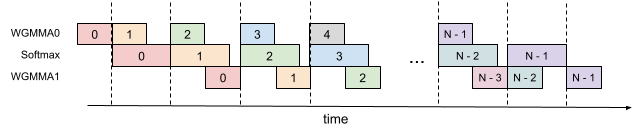
\includegraphics[width=.95\linewidth]{figs/3_stage_pipelining.png}
    \caption{3-Stage Pipelining}
    \label{fig:3_stage_pipelining}
\end{figure}

\begin{algorithm}[H]
    \caption{\small\label{alg:flash3_3_stage_wgmma}\sysnameone 3-stage pipelining consumer warpgroup forward pass}
    \begin{algorithmic}[1]
      \REQUIRE Matrices $\vQ, \vK, \vV \in \mathbb{R}^{N \times d}$ in HBM, block sizes $B_c$, $B_r$.
      Each warpgroup reads 1 block Qi of size $B_r \times d$, $T_c = \left\lceil \frac{N}{B_c} \right\rceil$ blocks $\vK_1, \dots, \vK_{T_c}$ and
      $\vV_1, \dots, \vV_{T_c}$ of size $B_c \times d$.
      Each warpgroup writes 1 output block $\vO_i$ of size $B_r \times d$, and 1 logsumexp block $L_i$ of size $B_r$.
      \STATE Initialization. Load $\vQ_i$ from HBM to on-chip SRAM.
      Initialize $\vO_{i}, \ell_{i}, m_{i}, scale\_o$.
      \STATE Wait for the producer warpgroup loading $\vK_0$ from HBM to on-chip SRAM.
      \STATE Compute $\vS = \vQ_i \vK_0^T$ using WGMMA. Commit and wait.
      \STATE Compute $m_{i}$, $\tilde{\vP}_{i}$, $\ell_{i}$, $scale\_o$ based on $\vS$.
      \STATE Wait for the producer warpgroup loading $\vK_1$ from HBM to on-chip SRAM.
      \STATE Compute $\vS = \vQ_i \vK_1^T$ using WGMMA. Commit and wait.
      \FOR{$2 \le j < T_c - 2$}
        \STATE Wait for the producer warpgroup loading $\vK_j$ from HBM to on-chip SRAM.
        \STATE Compute $\vS\_next = \vQ_i \vK_{j}^T$ using WGMMA. Commit but do not wait.
        \STATE Wait for the producer warpgroup loading $\vV_{j-2}$ from HBM to on-chip SRAM.
        \STATE Rescale $\vO_{i}$ based on $scale\_o$.
        \STATE Compute
        $\vO_{i} = \vO_{i} + \tilde{\vP}_{i} \vV_{j-2}$ using WGMMA. Commit but do not wait.
        \STATE Compute $m_{i}$, $\tilde{\vP}_{i}\_next$, $\ell_{i}$, $scale\_o$ based on $\vS$.
        \STATE Wait for all previous WGMMAs.
        \STATE Copy $\vS\_next$ to $\vS$.
        \STATE Copy $\tilde{\vP}_{i}\_next$ to $\tilde{\vP}_{i}$.
      \ENDFOR
      \STATE Wait for the producer warpgroup loading $\vV_{T_c-2}$ from HBM to on-chip SRAM.
      \STATE Rescale $\vO_{i}$ based on $scale\_o$.
      \STATE Compute
      $\vO_{i} = \vO_{i} + \tilde{\vP}_{i} \vV_{T_c-2}$ using WGMMA. Commit and wait.
      \STATE Compute $m_{i}$, $\tilde{\vP}_{i}$, $\ell_{i}$, $scale\_o$ based on $\vS$.
      \STATE Wait for the producer warpgroup loading $\vV_{T_c-1}$ from HBM to on-chip SRAM.
      \STATE Rescale $\vO_{i}$ based on $scale\_o$.
      \STATE Compute
      $\vO_{i} = \vO_{i} + \tilde{\vP}_{i} \vV_{T_c-1}$ using WGMMA. Commit and wait.
      \STATE Epilogue. Rescale $\vO_{i}$ based on $\ell_{i}$. Compute $L_{i}$ based on $\ell_{i}$ and $m_{i}$. Write $\vO_{i}$ and $L_{i}$ to HBM as the $i$-th block of $\vO$ and $L$.
    \end{algorithmic}
  \end{algorithm}

\paragraph{Overlapping.} 
We expected that softmax can be overlapped with (the first WGMMA + the second WGMMA). However, the compiler doesn't cooperate in this way.
SASS code shows that only the first WGMMA is overlapped with softmax, while the second WGMMA is not. It's not clear why the compiler chooses to reorder instructions in this way.

\paragraph{Register pressure.}
This algorithm requires more registers compared to the 2-stage pipelining algorithm. 
In theory, it needs to store an extra $\tilde{\vP}_{i}$ and $scale\_o$, which is of size $B_r \times B_c \times \text{sizeof}(\text{input\_data\_type}) + B_r \times \text{sizeof}(\text{float})$.
As a result, a smaller block size needs to be chosen.














\section{Addition Details on Experiments and Benchmarking}

\subsection{System and libraries}
\label{sec:system}

We benchmark the speed on an H100 80GB SXM5 (700W).
We generally use the latest versions of the libraries, at the time of writing
(May 2024).
Specifically, we use:
\begin{itemize}
\item CUDA 12.3
\item cuDNN 9.1.1.17
\item CUTLASS 3.5
\item \fa 2.5.8
\item Triton nightly 3.0.0.post20240424212437
\item PyTorch 2.3.0
\end{itemize}

To reduce variability, we fix the GPU clock speed to 1830MHz (clock speed used
to calculate the 989 TFLOPS FP16 theoretical max throughput).
We repeat the benchmarks 100 times and take the average timing.






\subsection{FP8 Attention Full Results}
\label{sec:benchmark_attn_fp8_full}

We use following sequence lengths: 512, 1024, 2048, 4224, 8448, 16896.
When sequence length $\geq$ 4k, we make it also divisible by 132 (number of SMs in H100 SXM5) to avoid wave quantization.

\begin{figure}[ht]
  \centering
  \begin{subfigure}{.5\textwidth}
    \centering
    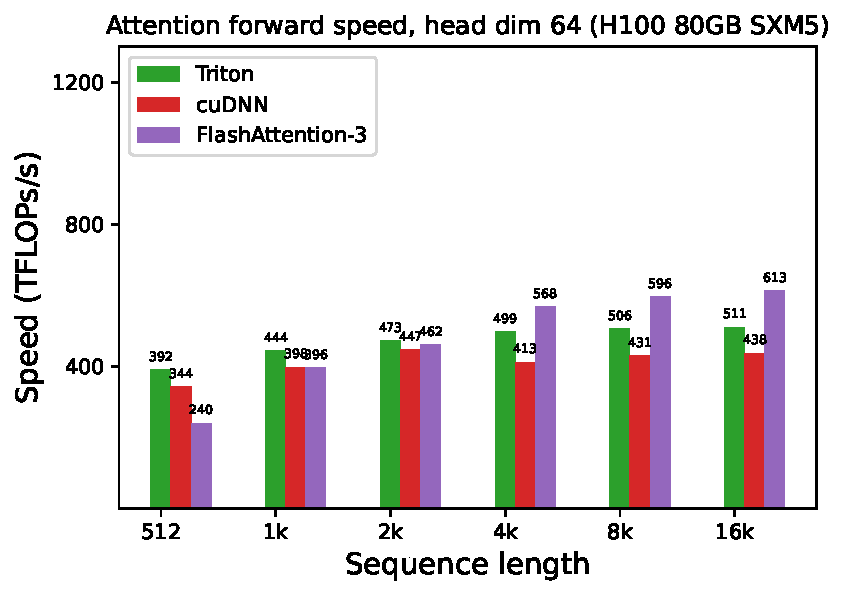
\includegraphics[width=.95\linewidth]{figs/flash3_h100_fp8_causal_False_hdim_64_fwd_speed.pdf}
    \caption{Forward, without causal mask, head dim 64}
  \end{subfigure}%
  \begin{subfigure}{.5\textwidth}
    \centering
    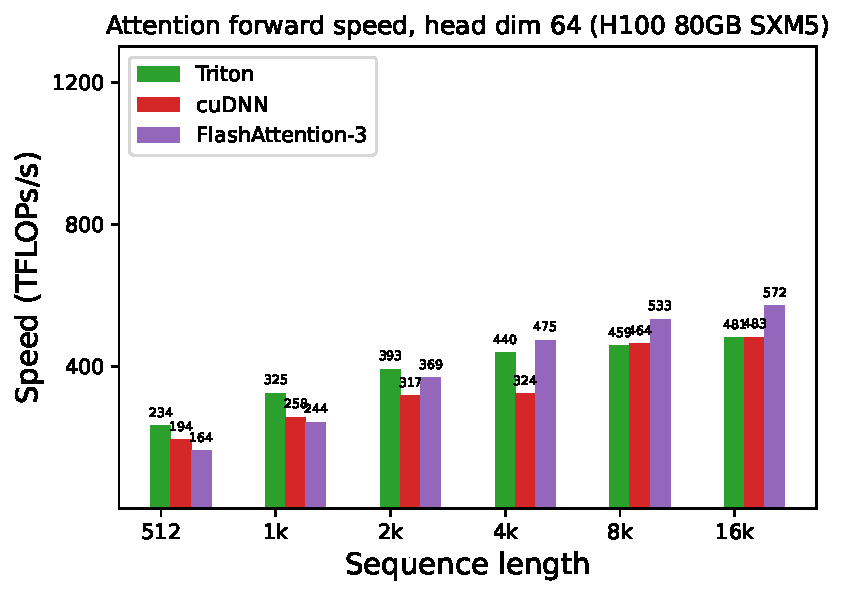
\includegraphics[width=.95\linewidth]{figs/flash3_h100_fp8_causal_True_hdim_64_fwd_speed.pdf}
    \caption{Forward, with causal mask, head dim 64}
  \end{subfigure}
  \begin{subfigure}{.5\textwidth}
    \centering
    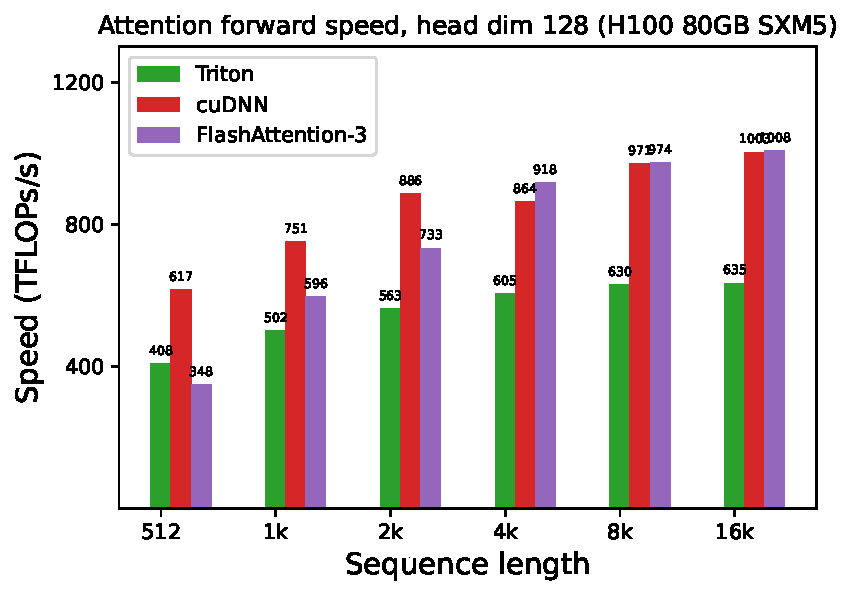
\includegraphics[width=.95\linewidth]{figs/flash3_h100_fp8_causal_False_hdim_128_fwd_speed.pdf}
    \caption{Forward, without causal mask, head dim 128}
  \end{subfigure}%
  \begin{subfigure}{.5\textwidth}
    \centering
    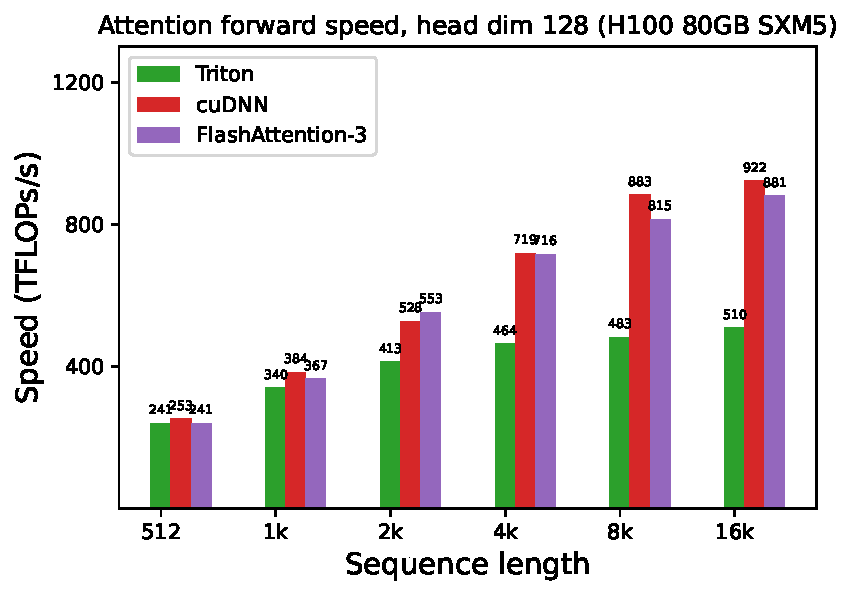
\includegraphics[width=.95\linewidth]{figs/flash3_h100_fp8_causal_True_hdim_128_fwd_speed.pdf}
    \caption{Forward, with causal mask, head dim 128}
  \end{subfigure}
  \begin{subfigure}{.5\textwidth}
    \centering
    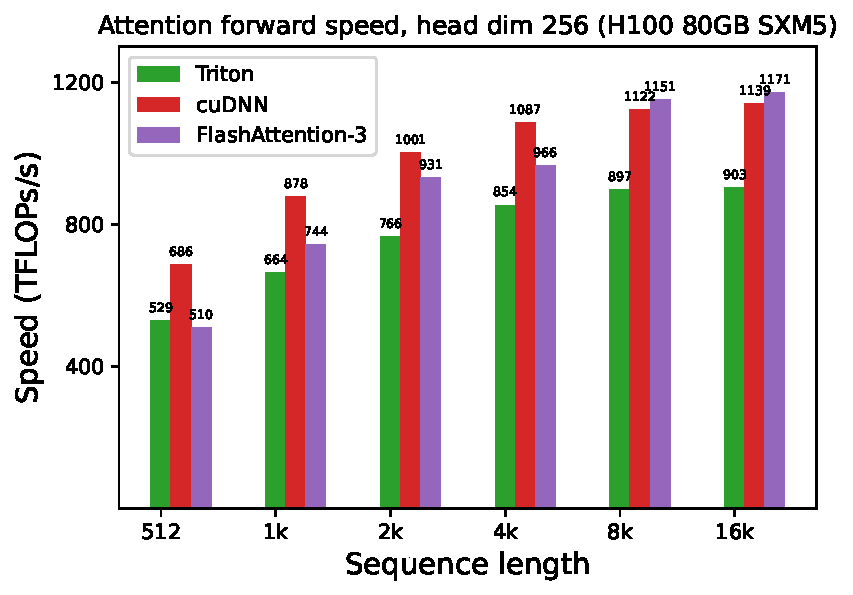
\includegraphics[width=.95\linewidth]{figs/flash3_h100_fp8_causal_False_hdim_256_fwd_speed.pdf}
    \caption{Forward, without causal mask, head dim 256}
  \end{subfigure}%
  \begin{subfigure}{.5\textwidth}
    \centering
    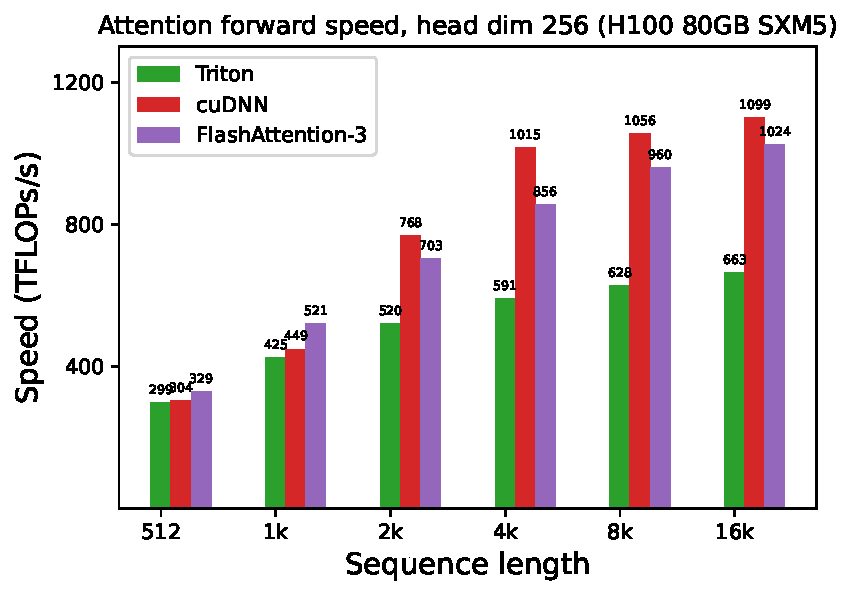
\includegraphics[width=.95\linewidth]{figs/flash3_h100_fp8_causal_True_hdim_256_fwd_speed.pdf}
    \caption{Forward, with causal mask, head dim 256}
  \end{subfigure}
  \caption{Attention forward speed (FP8) on H100 GPU}
  \label{fig:benchmark_attn_fwd_full}
\end{figure}


\iftoggle{arxiv}{}{
\newpage
\section*{NeurIPS Paper Checklist}

\begin{enumerate}

\item {\bf Claims}
    \item[] Question: Do the main claims made in the abstract and introduction accurately reflect the paper's contributions and scope?
    \item[] Answer: \answerYes{} 
    \item[] Justification: The abstract and the introduction both clearly state the claims made by the paper, along with a clear description of the contributions, assumptions and limitations. 
    \item[] Guidelines:
    \begin{itemize}
        \item The answer NA means that the abstract and introduction do not include the claims made in the paper.
        \item The abstract and/or introduction should clearly state the claims made, including the contributions made in the paper and important assumptions and limitations. A No or NA answer to this question will not be perceived well by the reviewers. 
        \item The claims made should match theoretical and experimental results, and reflect how much the results can be expected to generalize to other settings. 
        \item It is fine to include aspirational goals as motivation as long as it is clear that these goals are not attained by the paper. 
    \end{itemize}

\item {\bf Limitations}
    \item[] Question: Does the paper discuss the limitations of the work performed by the authors?
    \item[] Answer: \answerYes{}
    \item[] Justification: Yes, the limitations of the current work as well as the avenues for future improvements to the current work can be found in Section \ref{sec:disc}.
    \item[] Guidelines:
    \begin{itemize}
        \item The answer NA means that the paper has no limitation while the answer No means that the paper has limitations, but those are not discussed in the paper. 
        \item The authors are encouraged to create a separate "Limitations" section in their paper.
        \item The paper should point out any strong assumptions and how robust the results are to violations of these assumptions (e.g., independence assumptions, noiseless settings, model well-specification, asymptotic approximations only holding locally). The authors should reflect on how these assumptions might be violated in practice and what the implications would be.
        \item The authors should reflect on the scope of the claims made, e.g., if the approach was only tested on a few datasets or with a few runs. In general, empirical results often depend on implicit assumptions, which should be articulated.
        \item The authors should reflect on the factors that influence the performance of the approach. For example, a facial recognition algorithm may perform poorly when image resolution is low or images are taken in low lighting. Or a speech-to-text system might not be used reliably to provide closed captions for online lectures because it fails to handle technical jargon.
        \item The authors should discuss the computational efficiency of the proposed algorithms and how they scale with dataset size.
        \item If applicable, the authors should discuss possible limitations of their approach to address problems of privacy and fairness.
        \item While the authors might fear that complete honesty about limitations might be used by reviewers as grounds for rejection, a worse outcome might be that reviewers discover limitations that aren't acknowledged in the paper. The authors should use their best judgment and recognize that individual actions in favor of transparency play an important role in developing norms that preserve the integrity of the community. Reviewers will be specifically instructed to not penalize honesty concerning limitations.
    \end{itemize}

\item {\bf Theory Assumptions and Proofs}
    \item[] Question: For each theoretical result, does the paper provide the full set of assumptions and a complete (and correct) proof?
    \item[] Answer: \answerYes{} 
    \item[] Justification: Yes, for all the main results of the paper in Section \ref{sec:eigenspectrum_theory}, a full set of assumptions and a complete proof is provided in Section \ref{app:sec_proof} in the Appendix. 
    \item[] Guidelines:
    \begin{itemize}
        \item The answer NA means that the paper does not include theoretical results. 
        \item All the theorems, formulas, and proofs in the paper should be numbered and cross-referenced.
        \item All assumptions should be clearly stated or referenced in the statement of any theorems.
        \item The proofs can either appear in the main paper or the supplemental material, but if they appear in the supplemental material, the authors are encouraged to provide a short proof sketch to provide intuition. 
        \item Inversely, any informal proof provided in the core of the paper should be complemented by formal proofs provided in appendix or supplemental material.
        \item Theorems and Lemmas that the proof relies upon should be properly referenced. 
    \end{itemize}

    \item {\bf Experimental Result Reproducibility}
    \item[] Question: Does the paper fully disclose all the information needed to reproduce the main experimental results of the paper to the extent that it affects the main claims and/or conclusions of the paper (regardless of whether the code and data are provided or not)?
    \item[] Answer: \answerYes{} 
    \item[] Justification: Yes, the paper discloses all the necessary details about the implemented architectures used, hyperparameters for each setting, algorithm pseudocode and other experimental details to reproduce all the experiments in the paper. These details can be found in Section \ref{app:secB} in the Appendix.
    \item[] Guidelines:
    \begin{itemize}
        \item The answer NA means that the paper does not include experiments.
        \item If the paper includes experiments, a No answer to this question will not be perceived well by the reviewers: Making the paper reproducible is important, regardless of whether the code and data are provided or not.
        \item If the contribution is a dataset and/or model, the authors should describe the steps taken to make their results reproducible or verifiable. 
        \item Depending on the contribution, reproducibility can be accomplished in various ways. For example, if the contribution is a novel architecture, describing the architecture fully might suffice, or if the contribution is a specific model and empirical evaluation, it may be necessary to either make it possible for others to replicate the model with the same dataset, or provide access to the model. In general. releasing code and data is often one good way to accomplish this, but reproducibility can also be provided via detailed instructions for how to replicate the results, access to a hosted model (e.g., in the case of a large language model), releasing of a model checkpoint, or other means that are appropriate to the research performed.
        \item While NeurIPS does not require releasing code, the conference does require all submissions to provide some reasonable avenue for reproducibility, which may depend on the nature of the contribution. For example
        \begin{enumerate}
            \item If the contribution is primarily a new algorithm, the paper should make it clear how to reproduce that algorithm.
            \item If the contribution is primarily a new model architecture, the paper should describe the architecture clearly and fully.
            \item If the contribution is a new model (e.g., a large language model), then there should either be a way to access this model for reproducing the results or a way to reproduce the model (e.g., with an open-source dataset or instructions for how to construct the dataset).
            \item We recognize that reproducibility may be tricky in some cases, in which case authors are welcome to describe the particular way they provide for reproducibility. In the case of closed-source models, it may be that access to the model is limited in some way (e.g., to registered users), but it should be possible for other researchers to have some path to reproducing or verifying the results.
        \end{enumerate}
    \end{itemize}


\item {\bf Open access to data and code}
    \item[] Question: Does the paper provide open access to the data and code, with sufficient instructions to faithfully reproduce the main experimental results, as described in supplemental material?
    \item[] Answer: \answerYes{} 
    \item[] Justification: The paper includes the specific instructions to access the datasets used for all the experimentation. These can be found in Section \ref{app:secB} in the Appendix. The code for this project is released to the public. 
    \item[] Guidelines:
    \begin{itemize}
        \item The answer NA means that paper does not include experiments requiring code.
        \item Please see the NeurIPS code and data submission guidelines (\url{https://nips.cc/public/guides/CodeSubmissionPolicy}) for more details.
        \item While we encourage the release of code and data, we understand that this might not be possible, so “No” is an acceptable answer. Papers cannot be rejected simply for not including code, unless this is central to the contribution (e.g., for a new open-source benchmark).
        \item The instructions should contain the exact command and environment needed to run to reproduce the results. See the NeurIPS code and data submission guidelines (\url{https://nips.cc/public/guides/CodeSubmissionPolicy}) for more details.
        \item The authors should provide instructions on data access and preparation, including how to access the raw data, preprocessed data, intermediate data, and generated data, etc.
        \item The authors should provide scripts to reproduce all experimental results for the new proposed method and baselines. If only a subset of experiments are reproducible, they should state which ones are omitted from the script and why.
        \item At submission time, to preserve anonymity, the authors should release anonymized versions (if applicable).
        \item Providing as much information as possible in supplemental material (appended to the paper) is recommended, but including URLs to data and code is permitted.
    \end{itemize}


\item {\bf Experimental Setting/Details}
    \item[] Question: Does the paper specify all the training and test details (e.g., data splits, hyperparameters, how they were chosen, type of optimizer, etc.) necessary to understand the results?
    \item[] Answer: \answerYes{} 
    \item[] Justification: Yes, the paper uses standard data splits from publicly available benchmark sources and provides details regarding the choice of hyperparameters, optimizer and other decisions necessary for understanding the results. These details can be found in Section \ref{app:secB} in the Appendix.
    \item[] Guidelines:
    \begin{itemize}
        \item The answer NA means that the paper does not include experiments.
        \item The experimental setting should be presented in the core of the paper to a level of detail that is necessary to appreciate the results and make sense of them.
        \item The full details can be provided either with the code, in appendix, or as supplemental material.
    \end{itemize}

\item {\bf Experiment Statistical Significance}
    \item[] Question: Does the paper report error bars suitably and correctly defined or other appropriate information about the statistical significance of the experiments?
    \item[] Answer: \answerYes{} 
    \item[] Justification: Yes, the paper reports the error bars and other information about the statistical significance of the results in the Section \ref{sec:experiments} in the main paper. 
    \item[] Guidelines:
    \begin{itemize}
        \item The answer NA means that the paper does not include experiments.
        \item The authors should answer "Yes" if the results are accompanied by error bars, confidence intervals, or statistical significance tests, at least for the experiments that support the main claims of the paper.
        \item The factors of variability that the error bars are capturing should be clearly stated (for example, train/test split, initialization, random drawing of some parameter, or overall run with given experimental conditions).
        \item The method for calculating the error bars should be explained (closed form formula, call to a library function, bootstrap, etc.)
        \item The assumptions made should be given (e.g., Normally distributed errors).
        \item It should be clear whether the error bar is the standard deviation or the standard error of the mean.
        \item It is OK to report 1-sigma error bars, but one should state it. The authors should preferably report a 2-sigma error bar than state that they have a 96\% CI, if the hypothesis of Normality of errors is not verified.
        \item For asymmetric distributions, the authors should be careful not to show in tables or figures symmetric error bars that would yield results that are out of range (e.g. negative error rates).
        \item If error bars are reported in tables or plots, The authors should explain in the text how they were calculated and reference the corresponding figures or tables in the text.
    \end{itemize}

\item {\bf Experiments Compute Resources}
    \item[] Question: For each experiment, does the paper provide sufficient information on the computer resources (type of compute workers, memory, time of execution) needed to reproduce the experiments?
    \item[] Answer: \answerYes{} 
    \item[] Justification: Yes, the paper provides details about the compute resources, hardware and software needed to reproduce the experiments in Section \ref{app:secB} of the Appendix.
    \item[] Guidelines:
    \begin{itemize}
        \item The answer NA means that the paper does not include experiments.
        \item The paper should indicate the type of compute workers CPU or GPU, internal cluster, or cloud provider, including relevant memory and storage.
        \item The paper should provide the amount of compute required for each of the individual experimental runs as well as estimate the total compute. 
        \item The paper should disclose whether the full research project required more compute than the experiments reported in the paper (e.g., preliminary or failed experiments that didn't make it into the paper). 
    \end{itemize}
    
\item {\bf Code Of Ethics}
    \item[] Question: Does the research conducted in the paper conform, in every respect, with the NeurIPS Code of Ethics \url{https://neurips.cc/public/EthicsGuidelines}?
    \item[] Answer: \answerYes{} 
    \item[] Justification: Yes, the research conducted in this paper conforms in every respect, with the NeurIPS code of ethics. 
    \item[] Guidelines:
    \begin{itemize}
        \item The answer NA means that the authors have not reviewed the NeurIPS Code of Ethics.
        \item If the authors answer No, they should explain the special circumstances that require a deviation from the Code of Ethics.
        \item The authors should make sure to preserve anonymity (e.g., if there is a special consideration due to laws or regulations in their jurisdiction).
    \end{itemize}


\item {\bf Broader Impacts}
    \item[] Question: Does the paper discuss both potential positive societal impacts and negative societal impacts of the work performed?
    \item[] Answer: \answerYes{} 
    \item[] Justification: We discuss the potential positive and negative societal impacts of our work in Section \ref{app:broader_impact} of the Appendix. 
    \item[] Guidelines:
    \begin{itemize}
        \item The answer NA means that there is no societal impact of the work performed.
        \item If the authors answer NA or No, they should explain why their work has no societal impact or why the paper does not address societal impact.
        \item Examples of negative societal impacts include potential malicious or unintended uses (e.g., disinformation, generating fake profiles, surveillance), fairness considerations (e.g., deployment of technologies that could make decisions that unfairly impact specific groups), privacy considerations, and security considerations.
        \item The conference expects that many papers will be foundational research and not tied to particular applications, let alone deployments. However, if there is a direct path to any negative applications, the authors should point it out. For example, it is legitimate to point out that an improvement in the quality of generative models could be used to generate deepfakes for disinformation. On the other hand, it is not needed to point out that a generic algorithm for optimizing neural networks could enable people to train models that generate Deepfakes faster.
        \item The authors should consider possible harms that could arise when the technology is being used as intended and functioning correctly, harms that could arise when the technology is being used as intended but gives incorrect results, and harms following from (intentional or unintentional) misuse of the technology.
        \item If there are negative societal impacts, the authors could also discuss possible mitigation strategies (e.g., gated release of models, providing defenses in addition to attacks, mechanisms for monitoring misuse, mechanisms to monitor how a system learns from feedback over time, improving the efficiency and accessibility of ML).
    \end{itemize}
    
\item {\bf Safeguards}
    \item[] Question: Does the paper describe safeguards that have been put in place for responsible release of data or models that have a high risk for misuse (e.g., pretrained language models, image generators, or scraped datasets)?
    \item[] Answer: \answerNA{} 
    \item[] Justification: The paper uses publicly available datasets, and does not release any data or code that have a risk of misuse. 
    \item[] Guidelines:
    \begin{itemize}
        \item The answer NA means that the paper poses no such risks.
        \item Released models that have a high risk for misuse or dual-use should be released with necessary safeguards to allow for controlled use of the model, for example by requiring that users adhere to usage guidelines or restrictions to access the model or implementing safety filters. 
        \item Datasets that have been scraped from the Internet could pose safety risks. The authors should describe how they avoided releasing unsafe images.
        \item We recognize that providing effective safeguards is challenging, and many papers do not require this, but we encourage authors to take this into account and make a best faith effort.
    \end{itemize}

\item {\bf Licenses for existing assets}
    \item[] Question: Are the creators or original owners of assets (e.g., code, data, models), used in the paper, properly credited and are the license and terms of use explicitly mentioned and properly respected?
    \item[] Answer: \answerYes{} 
    \item[] Justification: We have appropriately cited the original owners of data and code which is used in the paper. 
    \item[] Guidelines:
    \begin{itemize}
        \item The answer NA means that the paper does not use existing assets.
        \item The authors should cite the original paper that produced the code package or dataset.
        \item The authors should state which version of the asset is used and, if possible, include a URL.
        \item The name of the license (e.g., CC-BY 4.0) should be included for each asset.
        \item For scraped data from a particular source (e.g., website), the copyright and terms of service of that source should be provided.
        \item If assets are released, the license, copyright information, and terms of use in the package should be provided. For popular datasets, \url{paperswithcode.com/datasets} has curated licenses for some datasets. Their licensing guide can help determine the license of a dataset.
        \item For existing datasets that are re-packaged, both the original license and the license of the derived asset (if it has changed) should be provided.
        \item If this information is not available online, the authors are encouraged to reach out to the asset's creators.
    \end{itemize}

\item {\bf New Assets}
    \item[] Question: Are new assets introduced in the paper well documented and is the documentation provided alongside the assets?
    \item[] Answer: \answerNA{} 
    \item[] Justification: The paper does not release any new assets. 
    \item[] Guidelines:
    \begin{itemize}
        \item The answer NA means that the paper does not release new assets.
        \item Researchers should communicate the details of the dataset/code/model as part of their submissions via structured templates. This includes details about training, license, limitations, etc. 
        \item The paper should discuss whether and how consent was obtained from people whose asset is used.
        \item At submission time, remember to anonymize your assets (if applicable). You can either create an anonymized URL or include an anonymized zip file.
    \end{itemize}

\item {\bf Crowdsourcing and Research with Human Subjects}
    \item[] Question: For crowdsourcing experiments and research with human subjects, does the paper include the full text of instructions given to participants and screenshots, if applicable, as well as details about compensation (if any)? 
    \item[] Answer: \answerNA{} 
    \item[] Justification: The paper does not involve crowdsourcing, nor research with human subjects.
    \item[] Guidelines:
    \begin{itemize}
        \item The answer NA means that the paper does not involve crowdsourcing nor research with human subjects.
        \item Including this information in the supplemental material is fine, but if the main contribution of the paper involves human subjects, then as much detail as possible should be included in the main paper. 
        \item According to the NeurIPS Code of Ethics, workers involved in data collection, curation, or other labor should be paid at least the minimum wage in the country of the data collector. 
    \end{itemize}

\item {\bf Institutional Review Board (IRB) Approvals or Equivalent for Research with Human Subjects}
    \item[] Question: Does the paper describe potential risks incurred by study participants, whether such risks were disclosed to the subjects, and whether Institutional Review Board (IRB) approvals (or an equivalent approval/review based on the requirements of your country or institution) were obtained?
    \item[] Answer: \answerNA{} 
    \item[] Justification: The paper does not involve crowdsourcing nor research with human subjects.
    \item[] Guidelines:
    \begin{itemize}
        \item The answer NA means that the paper does not involve crowdsourcing nor research with human subjects.
        \item Depending on the country in which research is conducted, IRB approval (or equivalent) may be required for any human subjects research. If you obtained IRB approval, you should clearly state this in the paper. 
        \item We recognize that the procedures for this may vary significantly between institutions and locations, and we expect authors to adhere to the NeurIPS Code of Ethics and the guidelines for their institution. 
        \item For initial submissions, do not include any information that would break anonymity (if applicable), such as the institution conducting the review.
    \end{itemize}

\end{enumerate}
}


\end{document}
